%%% Template para anotações de aula
%%% Feito por Daniel Campos com base no template de Willian Chamma que fez com base no template de  Mikhail Klassen



\documentclass[12pt,a4paper, brazil]{article}

%%%%%%% INFORMAÇÕES DO CABEÇALHO
\newcommand{\workingDate}{\textsc{\selectlanguage{spanish}\today}}
\newcommand{\userName}{curso 25/26}
\newcommand{\institution}{UAL}
\usepackage{researchdiary_png}
\usepackage{tcolorbox}


\begin{document}

\begin{center}
{\textbf {\Large Práctica extra: Análisis del firmware de un router}}\\[5mm]
{\large } \\[5mm]
\today\\[5mm] %% se quiser colocar data
\end{center}


\section{Análisis de seguridad hardware}

Nuestro entorno diario está repleto de dispositivos digitales, por tanto son suceptibles de ser atacados. ¿Cómo podemos prevenir que alguno de todos los dispositivos que nos rodean en nuestro día a día, tanto en casa como en el trabajo o universidad, en el autobus, coche, etc. puedan suponer una amenaza para nuestra integridad, seguridad y privacidad? La respuesta es llegando a la vulnerabilidad antes que aquel que quiera explotarla en su beneficio. Un ejemplo de los dispositivos más vulnerables y que apenas reciben auditorías de seguridad (desde el punto de vista del firmware) son los routers. La figura~\ref{fig:router} muestra un router TP-LINK como los que podemos encontrar en pymes, hogares, etc. En este documento pretendo mostrar cómo extraer y analizar el firmware de un sistema empotrado. 
\begin{figure}[htpb]
    \centering
    \caption{Router TP-LINK.}
    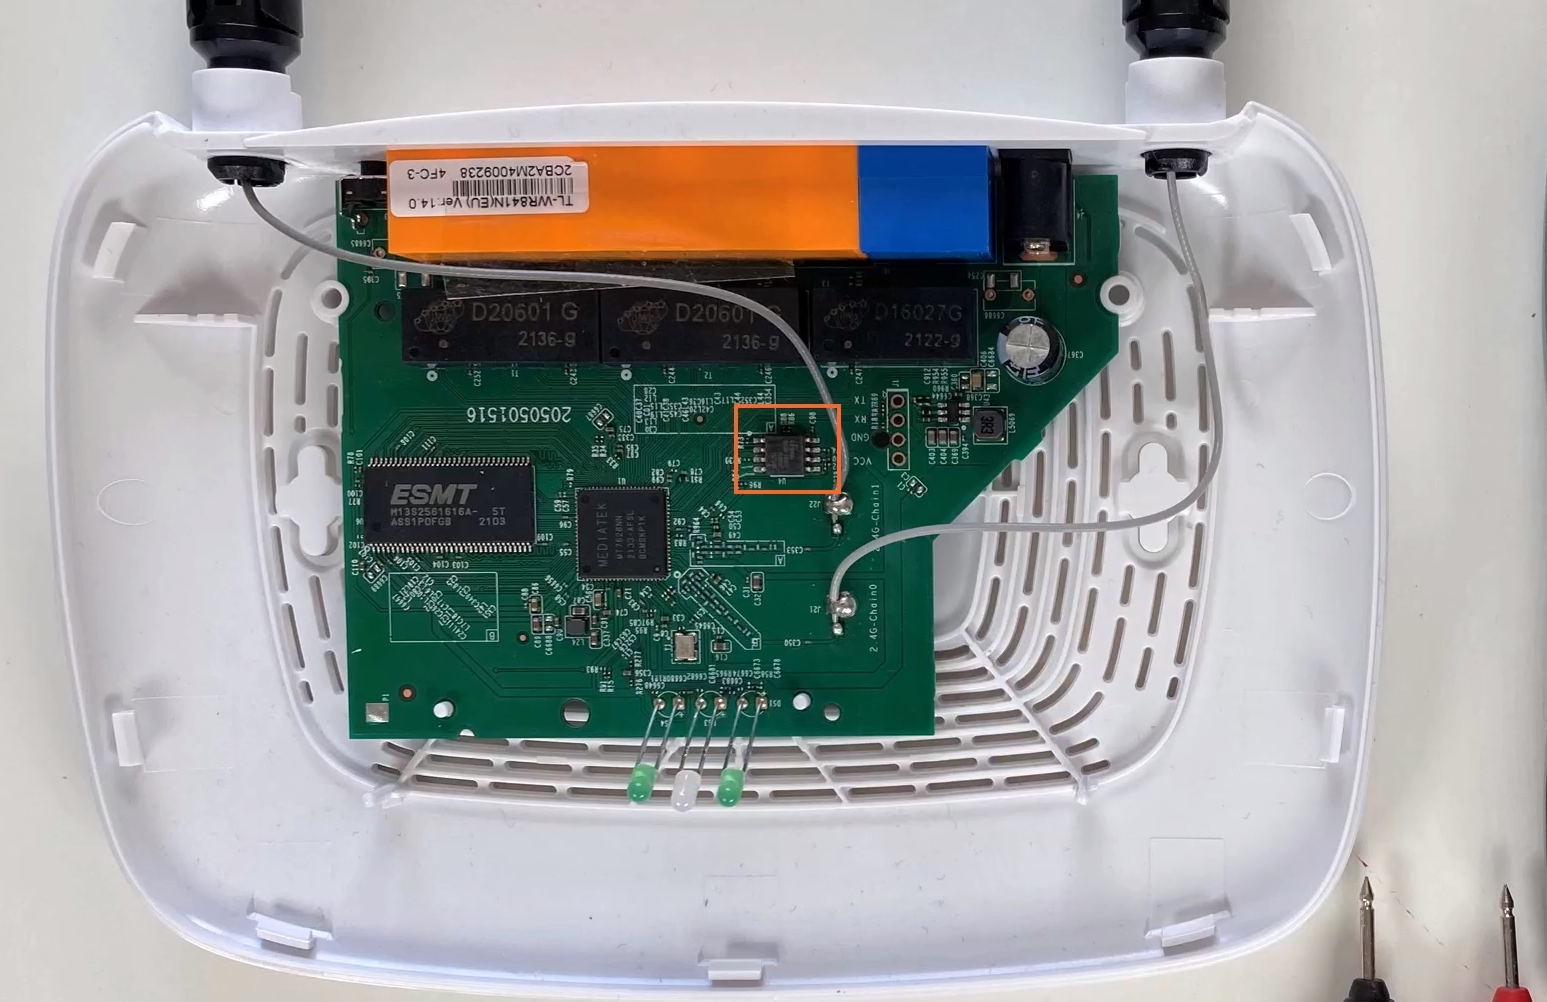
\includegraphics[scale=.2]{imagenes/1_router.png}
    \label{fig:router}
\end{figure}

La intención es estudiar si existen oportunidades de exfiltrado de información o amenazas mientras se usa el dispositivo. Los elementos básicos con los que vamos a trabajar se muestran en la figura~\ref{fig:accesorouter} donde se pueden ver los elementos usados para la extracción del firmware.
\begin{figure}[htpb]
    \centering
    \caption{Acceso al router.}
    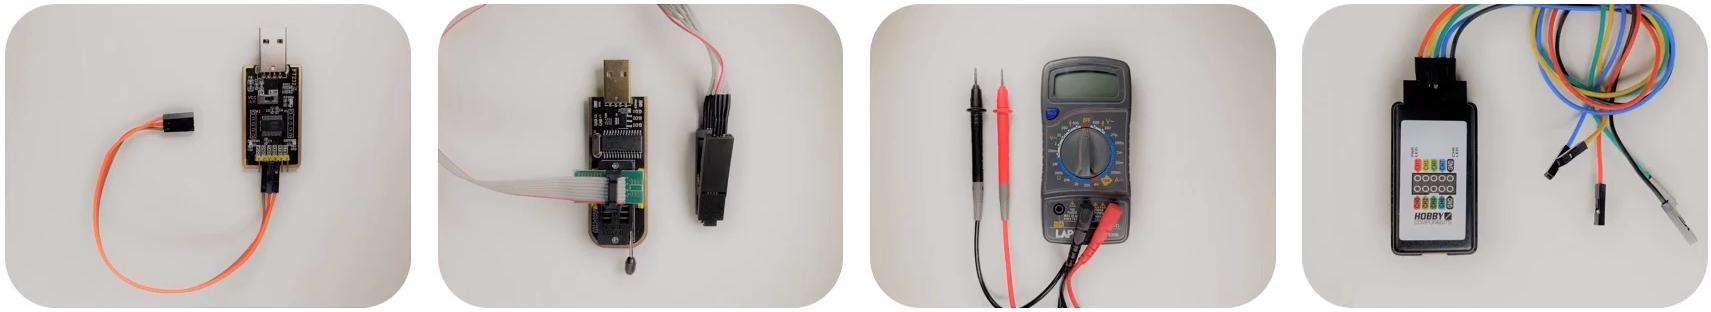
\includegraphics[scale=.25]{imagenes/1_accesorouter.png}
    \label{fig:accesorouter}
\end{figure}

En la figura~\ref{fig:router} hemos marcado intencionadamente uno de los chips (de los tres) con los que cuenta este dispositivo. Más adelante desarrollaremos los problemas que hemos encontrado y de las herramientas (con las que partimos) cuales hemos deshechado y cuales nos han servido finalmente. Cuando uno se enfrenta a un dispositivo como éste, el primer paso consiste en identificar los componentes y las interfaces de comunicación que éstos usan. Para ello es necesario documentarse antes. Por lo que en primer lugar y dependiendo de las intefaces de comunicación que nos ofrezca el dispositivo emplearemos unas técnicas (más lentas, como el acceso vía UART o los puertos de depuración) u otras más rápidas para tratar de acceder a lo que nos interesa: \emph{\textcolor{red}{firmware}}. 

Una vez que tengamos la información fuera del dispositivo el paso a seguir es conocer qué formato sigue toda la información binaria descargada. Es decir, ¿viene cifrada? ¿qué estructura tiene? ¿Cómo podemos abrir el paquete binario que acabamos -si es que tenemos éxito- de extraer del router? Para ello contaremos con un conjunto de herramientas (file carving, etc) que usaremos para tratar de averigurar con qué tipo de información estamos tratando y tratar de extraer información útil como el kernel y el sistema de archivos raíz (rootfs).  

La última etapa de este taller o práctica supone el uso de la ingeniería inversa (explicada en el capítulo titulado \emph{\textcolor{red}{reversing}}, en este caso hemos escogido \emph{\textcolor{red}{Ghidra}} frente a IDA) para ser capaces de extraer información útil tal como \emph{nombres de usuario, claves o hashes de las claves, claves de cifrado etc} para así tratar de identificar vulnerabilidades que podamos aprovechar. Hay que tener en cuenta que todos estos dispositivos cuentan con servidores internos que facilitan al usuario la configuración del mismo, y en este software es probable que existan problemas. 

\subsection{Ataques a través del hardware}
Todos somos conscientes de que en el desarrollo de aplicaciones pueden cometerse errores de programación (desde el punto de vista del \emph{\textcolor{red}{código seguro}} que pueda dar lugar a accesos no permitidos, esto lo hemos explorado en asignaturas como \emph{asignaturas de programación y de ingenieria del software} pero es cierto que el hardware supone un componente clave tabmbién, como aprendimos en \emph{Periféricos e Interfaces}, es posible que un criptosistema sea irrompible en la teoría pero su implementación descuidada en un SoC\footnote{System on Chip: dipositivo que cuenta con núcleos de procesamiento, memoria (sram, dram, flash) y microcontroladores, todo en el mismo encapsulado.} lo exponga y lo haga vulnerable. 

El análisis de \emph{pruebas de penetración o pentesting} es algo que es muy conocido por toda la comunidad de seguridad, y se entiende enfocado a redes y a servidores. Pero los dispositvos hardware son también una parte de la cadena que debe someterse a las pruebas de pentesting. En este caso se pretende analizar o localizar vulnerabilidades y la capacidad del hardware de impedir accesos no autorizados a través de interacciones físicas con el dispositivo. El procedimiento siempre sugiere que se \textbf{desmonte} el dispositivo (esto puede violar la garantía del mismo) y que se identifique dónde están las interfaces de depuración y/o comunicación, y podamos interactuar con ellas a bajo nivel. ¿Qué se persigue con esto? 
\begin{itemize}
    \item Analizar si el dispositivo se presta a revelar inforamción sensible: contraseñas, claves de cifrados, hashes almacenados en la memoria \emph{flash}. O si somos capaces de capturar esta información mientras se comunica internamente por los buses del sistema.
    \item Analizar si el dispositivo nos permite obtener una escalada de privilegios: consiste en analizar el software que se ejecuta en el dispositivo y considerar si podemos aprovechar que en ciertos momentos, este software, debe ganar acceso privilegiado y aprovecharlo para obtenerlo nosotros también.
    \item Analizar si habiendo ganado acceso a este dispositivo podemos compromenter otros que dependan de él. Esto es lo que se denomina \emph{pivotaje y movimiento lateral}.
\end{itemize}

La plétora de dispositivos que tenemos a nuestro alrededor es inmensa, y cada vez es mayor (así lo muestra la figura~\ref{fig:iot}. Los fabricantes, estresados por el TTM (Time To Market) apenas bastionan los firmware de los dispositivos. Haciendo que tanto ellos como el ecosistema al que se conecte sea extreamadamente vulnerable. 

\begin{figure}[htpb]
    \centering
    \caption{Ecosistema creciente de dispositivos.}
    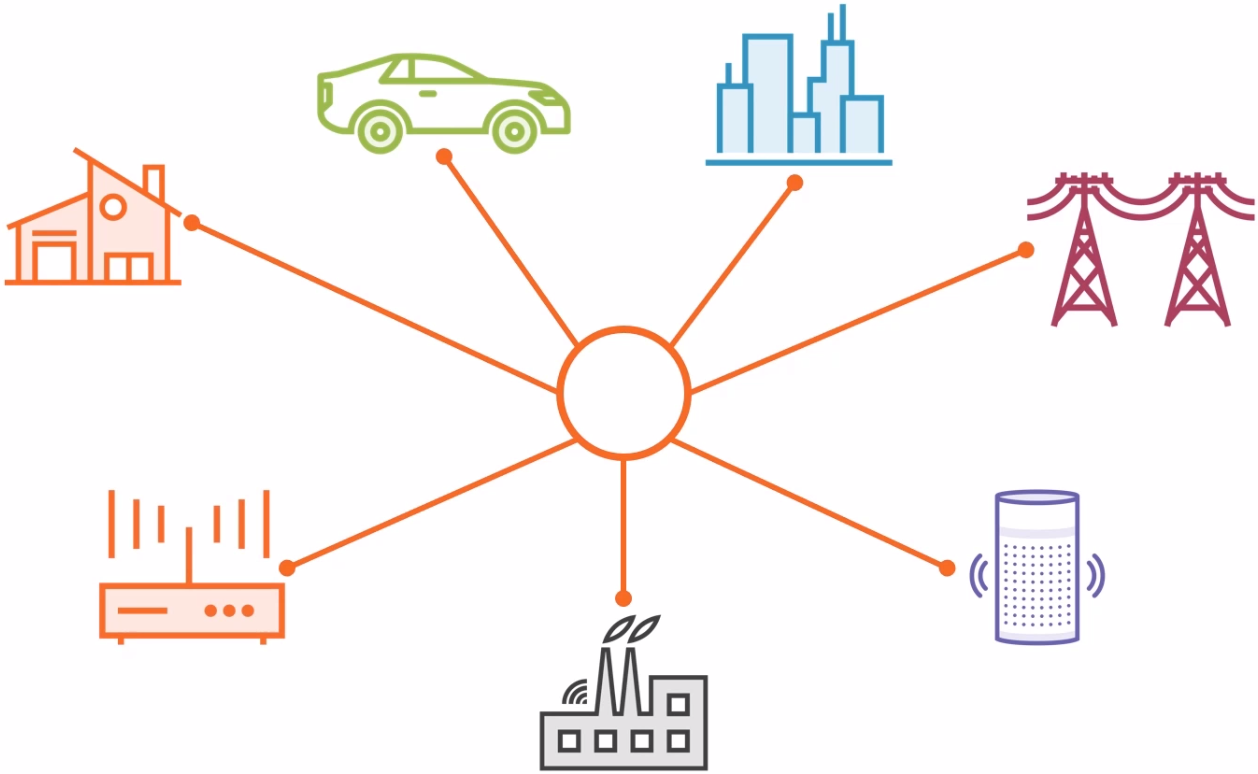
\includegraphics[scale=.25]{imagenes/1_ioT.png}
    \label{fig:iot}
\end{figure}

Todos estos dispositivos son ( y doy por sentado que lo serán ) suceptibles de ser atacados. Por tanto, disponer de técnicas para analizarlos y verificar su capacidad de protección es fundamental. Muchos de estos dispositivos emplean software que precisan de conexiones a internet (y a clouds corporativos) para permitir que el usuario (ya sea final o técnico -de la empresa, que realiza gestión sobre el dispositivo-) usan estas interfaces web para conectarse con el dispositivo, y esto incrementa aún más la superficie de exposición y ataque. Además estos dispositivos puede comunicarse a través de una amplia variedad de canales (Wi-Fi, Bluetooth, NFC, GSM, SMS etc) cada uno de estos protocolos tiene debilidades y vulnerabilidades conocidas, que a buen seguro van a ser usadas en contra de la integridad de nuestro dispositivo y los datos que protege. En este trabajo, vamos a realizar el análisis desde la capa física y no desde las aplicaciones y protocolos de red, que son el campo acostumbrado de las \emph{pruebas de penetración}. A través de la capa hardware vamos a tratar de extraer inforamción sensible desde la propia configuración del dispositivo (ver figura~\ref{fig:ini}).

\begin{figure}[htpb]
    \centering
    \caption{Acceso a través de la capa hardware.}
    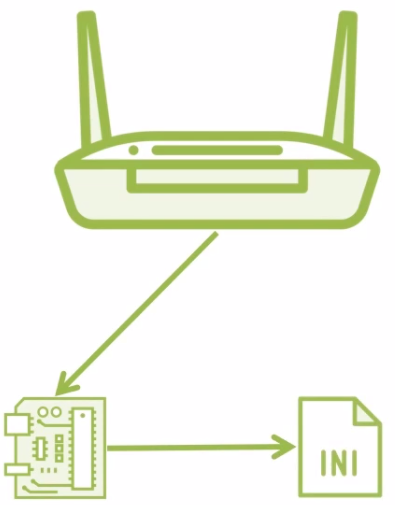
\includegraphics[scale=.3]{imagenes/1_ini.png}
    \label{fig:ini}
\end{figure}

\subsection{Identificación de componentes}

Ya hemos especificado en la sección anterior que este tipo de estudios requiere que se desmonte el dispositivo. Pero ¿cómo saber qué es lo que hay ahí conectado? ¿qué chips son esos? Para realizar este trabajo vamos a usar un router, moderno, adquirido vía \emph{amazon} y que podemos encontrar en hogares, tiedas pequeñas, etc. El router con el que vamos a trabajar es el \textbf{TL-WR841N}, como se muestra en la figura~\ref{fig:router} y se puede ver (tal como viene sin desmontar) en la figura~\ref{fig:routerTapa}:

\begin{figure}[htpb]
    \centering
    \caption{TL-WR841N}
    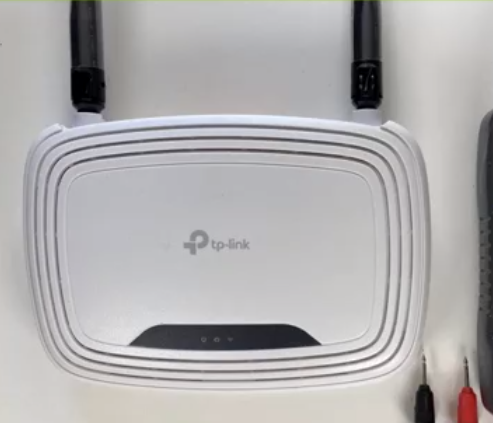
\includegraphics[scale=.4]{imagenes/1_routerTapa}
    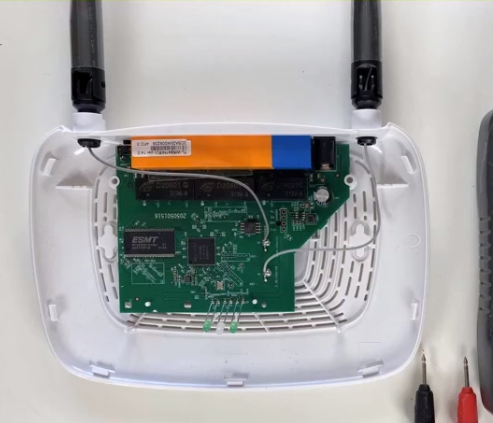
\includegraphics[scale=.4]{imagenes/1_routerTapa2}
    \label{fig:routerTapa}
\end{figure}

Es un router de 300Mbps, con interfaz cableada (ethernet) e inalámbrica (wi-fi). Hemos escogido este dipositivo por varias razones, en primer lugar por el \textbf{SoC} que incorpora (esto se desarrolla más adelante, en la sección de componentes) y en segundo lugar porque por sus capacidades técnicas se usa en muchos entornos (sobre todo pequeñas empresas), en último lugar porque por su precio, si el análisis termina inhabilitando el terminal, no habremos causado un daño apreciable. Para poder acceder a la placa, hemos de retirar dos tornillos en la parte inferior del dispositivo. Hecho esto, debemos retirar la tapa con cuidado porque está sujeta con pestañas de plástico. \textbf{\textcolor{red}{En la mayoría de los casos analizar un dispositivo como lo vamos a hacer, invalida la garantía y esto es algo que debe constar en la documentación si el análisis se va a realizar a terceros.}} Además, interaccionar con la circuitería de un dispositivo puede dañarlo por descuidos con la carga electrostática, por que causemos sin darnos cuenta cortocircuitos, por que le apliquemos más voltaje del que el dispositivo permite,etc. Por esto es útil tener un multimétro y la hoja técnica (datasheet) del dispositivo a mano. Al levantar la tapa, se muestran varios componentes:

\begin{itemize}
    \item \textbf{Banco de puertos ethernet (en naranja) y wan (en azul)}. Proporcionan la conectividad cableada al dispositivo). Ver figura~\ref{fig:ethernet}.
    \item \textbf{Alimentación del dispositivo}, que en este caso es una entrada en corriente continua de 9 voltios. Ver figura~\ref{fig:vcc}.
    \item \textbf{Interfaz serie}, usada para depuración del dispositivo. Consta de cuatro pines (\emph{transmisión (TX)}, \emph{recepción (RX)}, \emph{tierra (GND)} y \emph{alimentación (vcc)}). No es muy normal encontrar el etiquetado en las intefaces de depuración. En este caso, nos facilitan el trabajo, pero analizaremos las entradas igual que si no estuvieran marcadas para entender cómo identificar a qué corresponde cada pint. Ver figura~\ref{fig:depuracion}
    \item En la figura~\ref{fig:8bflash} podemos ver marcado un chip de memoria flash serie de 8 pines con capacidad de 32 Mb, consta de una interfaz serie para comunicarse con ella. \textbf{\textcolor{red}{Es en este chip donde vamos a encontrar almacenado el firmware del sistema}}. En un dispositivo tan sencillo como nuestro router, el \textbf{firmware} (\textbf{\textcolor{azul}{ya se ha explicado qué es y qué importancia tiene el firmware en secciones anteriores}}) proporciona el sistema operativo para que opere correctamente nuestro dispositivo. En dispositivos más complejos como PCs o portátiles, el firmware proporciona sólo las fase de arranque y carga del sistema, proporcionando una capa de abstracción.  
    \item \textbf{MediaTek MT7628 System On Chip (SoC)}. \textbf{\textcolor{red}{Este SoC es uno de los primeros SoCs diseñados y desarrollados especificamente para routers domésticos y para gateways IoT\footnote{Esto es especialmente relevante.}}} Esencialmente combina una radio Wi-Fi 802.11 con un procesador MIPS que trabaja a 580 MHz. 
    \item La figura~\ref{fig:memoria} muestra el último componente de interés, que es una memoria semiconductora de 4MB DDR SD-RAM.  Cuando el dispositivo arranque, el firmware caraga el sistema operativo desde la memoria flash en la ram (se ha explicado esto en la sección de firwmare inicial). Este proceso se denomina \emph{shadowing}. El sistema operativo está en la RAM hasta que se apaga el sistema. 
\end{itemize}

\begin{figure}[htpb]
    \centering
    \caption{Banco de puertos ethernet}
    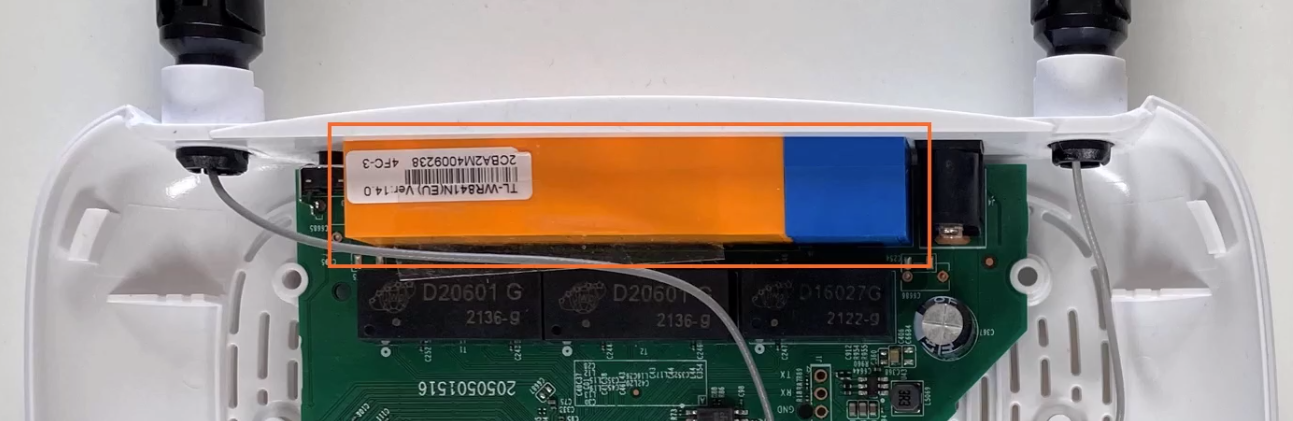
\includegraphics[scale=.4]{imagenes/1_ethernet.png}
    \label{fig:ethernet}
\end{figure}

\begin{figure}[htpb]
    \centering
    \caption{Alimentación: 9 voltios}
    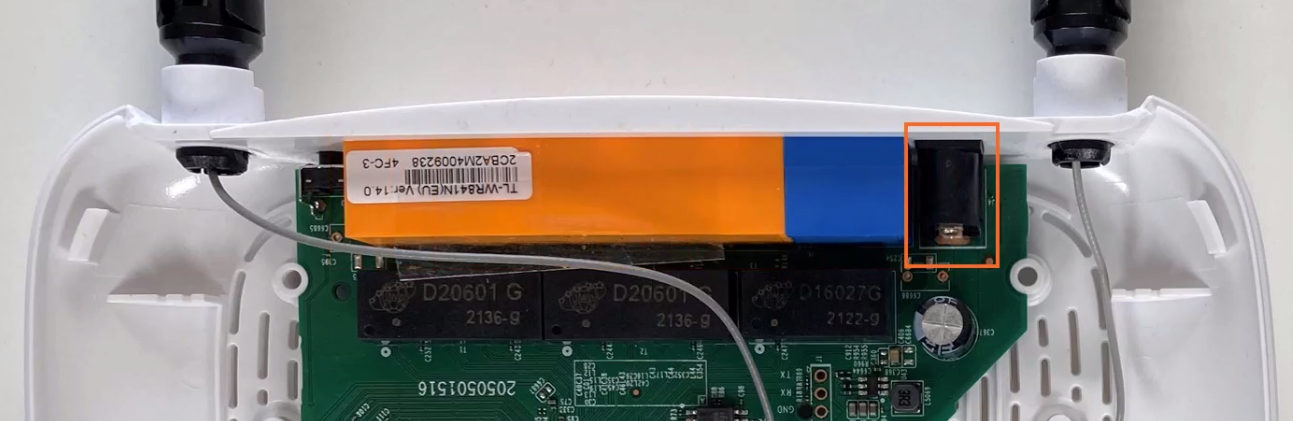
\includegraphics[scale=.4]{imagenes/1_vcc.png}
    \label{fig:vcc}
\end{figure}

\begin{figure}[htpb]
    \centering
    \caption{Interfaz serie de depuración}
    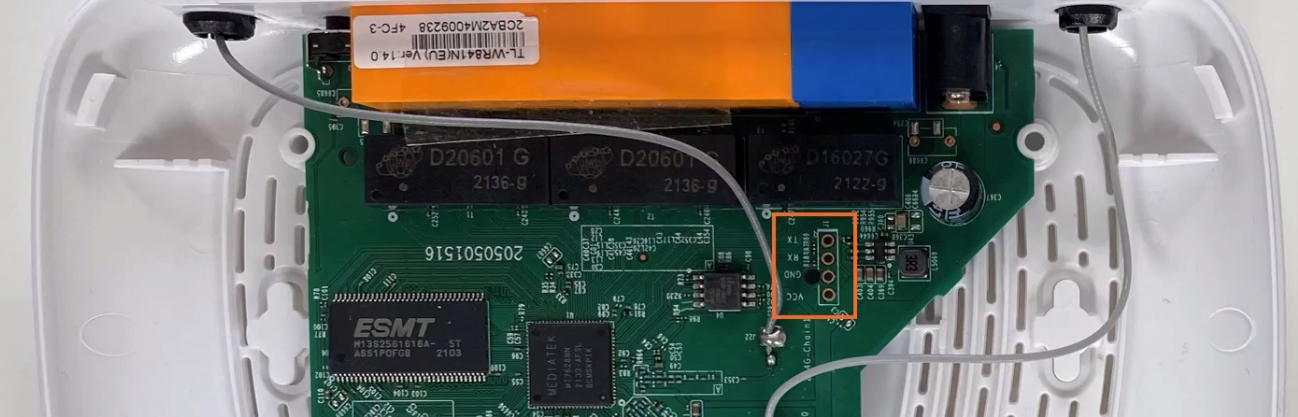
\includegraphics[scale=.4]{imagenes/1_depuracion.png}
    \label{fig:depuracion}
\end{figure}

\begin{figure}[htpb]
    \centering
    \caption{Memoria flash serie, de 8 bits. Hogar del firmware.}
    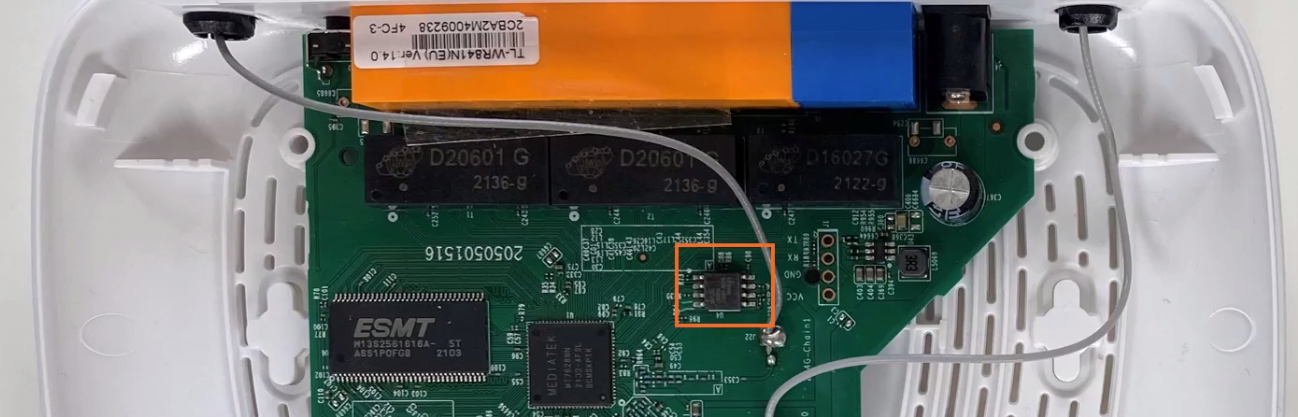
\includegraphics[scale=.4]{imagenes/1_8bflash.png}
    \label{fig:8bflash}
\end{figure}

\begin{figure}[htpb]
    \centering
    \caption{MediaTek MT7628 System On Chip (SoC).}
    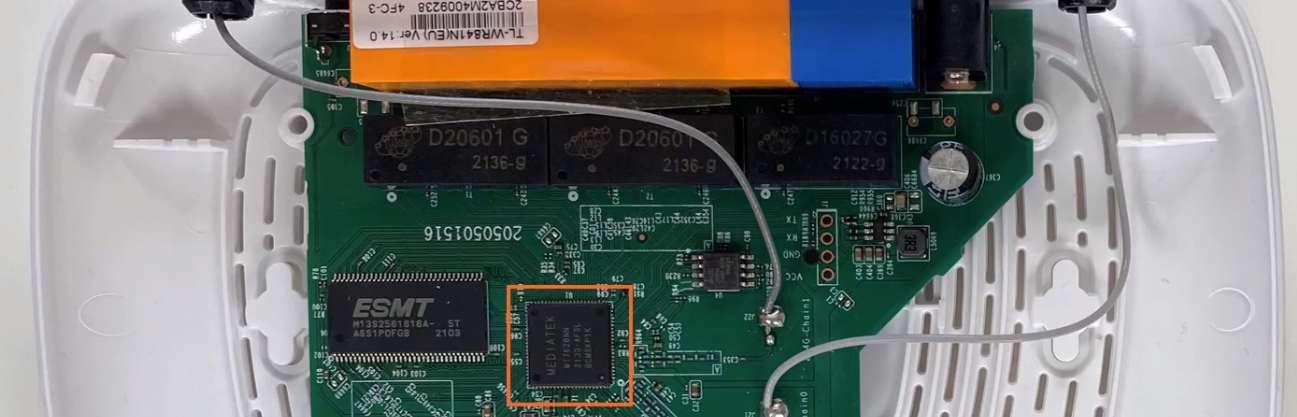
\includegraphics[scale=.4]{imagenes/1_soc.png}
    \label{fig:soc}
\end{figure}

\begin{figure}[htpb]
    \centering
    \caption{Memoria del sistema. DDR 4MB Elite SD-RAM}
    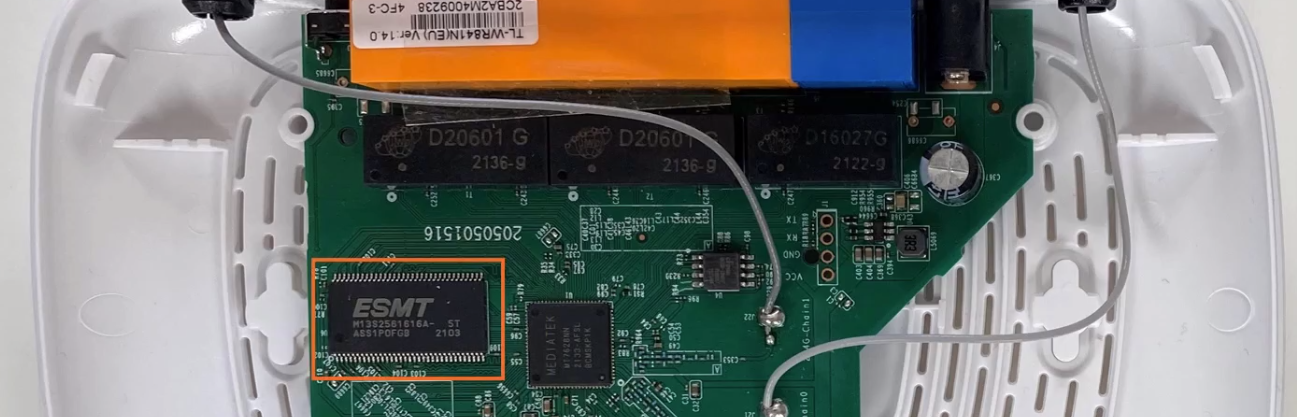
\includegraphics[scale=.4]{imagenes/1_memoria.png}
    \label{fig:memoria}
\end{figure}

Obviamente, es imposible simplemente mirando a los chips tras levantar la tapa, de qué marca y modelo son, cual es su función, etc. Pero si se emplean lupas o se amplifica se pueden extraer detalles de los chips (figura~\ref{fig:zoom}, que nos permitirá localizar su hoja de características técnicas. 

\begin{figure}[htpb]
    \centering
    \caption{Componentes}
    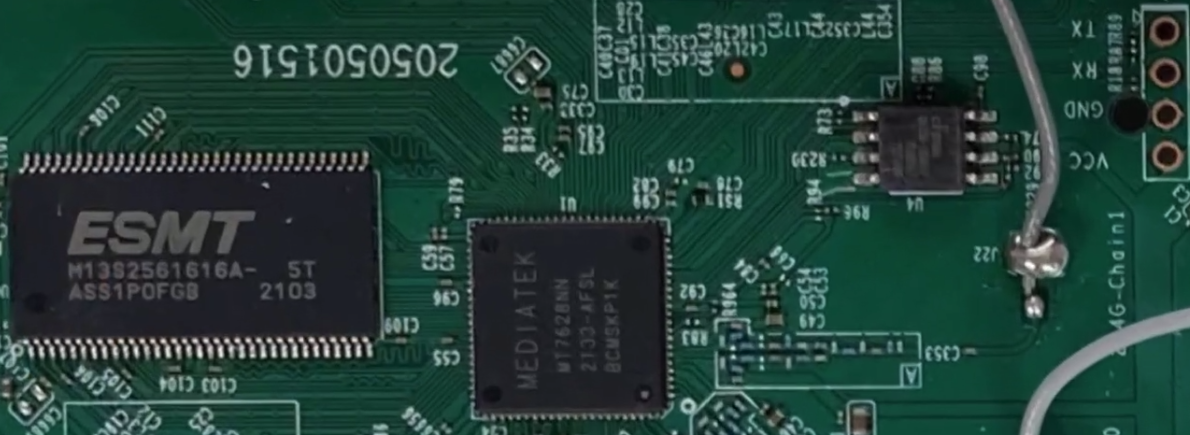
\includegraphics[scale=.4]{imagenes/1_zoom.png}
    \label{fig:zoom}
\end{figure}

\subsubsection{Interfaces}

Una vez que tenemos identificados a nuestros componentes fundamentales, la cuestión es saber con qué interfaces contamos para poder comunicarnos con ellos. En este router, la interfaz de depuración usa la \textbf{interfaz UART} (Universal Asynchornous Reciver Transmiter). Es una interfaz muy lenta. Proporciona una comunicación serie asíncrona (sin señal de reloj). Por tanto tiene una fase de configuración donde se establecen la velocidad y el formato de las tramas de datos. De modo que si usaramos estos pines, debemos configurar estos parámetros. La transmisión se realiza a través de dos líneas (pines) separados (el de transmisión y el de recepción). Sabemos, por tanto, que la interfaz de depuración usa UART. Por otro lado, al contar con una memoria flash NOR, la interfaz que se suele usar es la SPI. Aspecto que confirmamos al analizar el tipo de chip. 

\textbf{Interfaz SPI}: Al contrario que con UART (que es un cirtuito dentro del chip), SPI es un protocolo de comunicación, que sigue el modelo de comunicación cliente-servidor. SPI precisa de cuatro lineas de comunicación: una para que el cliente se comunique con el servidor (MISO), otra para que el servidor se comunique con el cliente (MOSI), otra para la señal de reloj (SCLK) , y la cuarta para seleccionar el servidor (chip) con el que comunicarnos (CS). 

\textbf{I2C (Inter-integrated circuit):} combina las mejores cualidades de UART con las mejores cualidades de SPI. De modo que podemos conectar varios servidores con un único cliente como con SPI y podemos tener a varios clientes controlando uno o varios servidores. Como UART, I2C, usa dos lineas de comunicación (SDA y SCL). El SDA o Serial Data line permite que tanto el servidor como el cliente envíen o reciban datos (half-duplex), SCL (serial clock) transporta la sincronización. 

\subsection{Herramientas}

En esta sección vamos a describir las herramientas que vamos (o que apriori pensamos) que pueden resultar útil para comunicarnos, interrogar, analizar a cada componente hardware. Considerando que contamos con una \textbf{interfaz UART}, la manera más sencilla de comunicarse a través de ésta interfaz es a través de un cable USB a TTL (figura~\ref{fig:usbttl}). 

\begin{figure}[htpb]
    \centering
    \caption{Herramientas: usb a ttl (FT232)}
    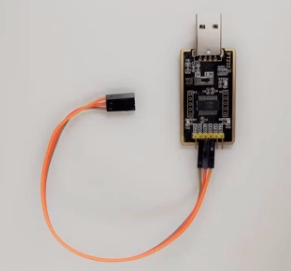
\includegraphics[scale=.6]{imagenes/1_usbttl.png}
    \label{fig:usbttl}
\end{figure}

Tal como se aprecia en la figura~\ref{fig:usbttl}, el cable contiene cuatro hilos, para conectar vcc, gnd, tx y rx. En el otro extremo tiene un conector USB, para conectarlo a un ordenador. 

Otra herramienta que nos va a resultar útil es el \textbf{programador de memorias flash} (figura~\ref{fig:flash}). Esta herraienta nos permite leer y/o escribir en memorias flash. en este caso hemos optado por un programador CH341A. 

\begin{figure}[htpb]
    \centering
    \caption{Herramientas: programador flash (CH341A).}
    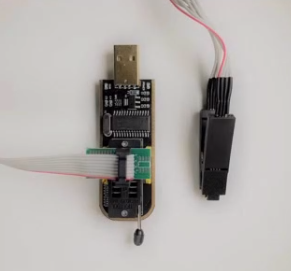
\includegraphics[scale=.6]{imagenes/1_flash.png}
    \label{fig:flash}
\end{figure}

En esta herramienta, hay que notar que porta una pinza para poder conectarse al chip en cuestión. Este programador puede escribir en flash vacías e incluso si el chip se retira de una placa, puede conectarse al programador y leerse directamente. En este caso, contamos con una pequeña faja (cable) que conecta el programador a un pequeño circuito de 8 pines (pinza SOIC). Esta pinza se conecta directamente al chip de memoria. Haciendo que cada pin del chip de memoria coincida con el pin correspondiente de la pinza. 

\textbf{Multimetro}: En la figura~\ref{fig:accesorouter} se muestran todas las herramientas que hemos usado, en esta figura se muestra el multimetro, cuya descripción es de todos ya conocida. En este caso vamos a usar el multímetro (ese en concreto) para indagar qué pines hemos de usar como recepción y como transmisión. 

\textbf{Analizador lógico}: A pesar de contar con uno, no ha sido finalmente necesario usarlo. Se emplean para analizar protocolos. La figura~\ref{fig:analizador} muestra el analizador (muy barato) que tenemos. Un analizador sirve para analizar señales en un sistema digital o circuito digital. 

\begin{figure}[htpb]
    \centering
    \caption{Herramientas: analizador lógico.}
    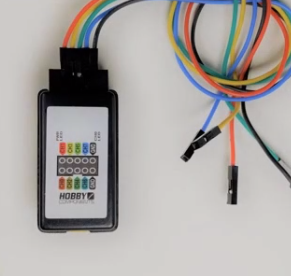
\includegraphics[scale=.6]{imagenes/1_analizador.png}
    \label{fig:analizador}
\end{figure}

El presupuesto invertido en adquirir estas herramientas no ha excedido los cuarenta euros. Por supuesto, el análisis de hardware requiere de herramientas profesionales cuyo presupuesto está muy por encima del que hemos usado. 

\subsubsection{Software}

Ahora que conocemos la arquitectura de nuestro dispositivo, que conocemos las interfaces que podemos usar para comuncarnos con él y que disponemos de un conjunto de herramientas básico, hay que analizar qué software podemos usar para emplear cada una de estas herramientas para poder realizar conexiones físicas con nuestro dispositivo. No hay una solución única, pero este conjunto de herramientas que exponemos es el tooblbox que es factible utilizar con las herramienta de que disponemos: 

\begin{itemize}
    \item \textbf{PuTTY}
    Emulador de terminal open source. Se diseñó originalmente para conexiones vía SSH, telnet y servicios similares con fines de administración remota. También permite comunicación serie. Para conectarnos a un dispositivo hemos de conocer la velocidad de transmisión (baud rate) para la que ha sido configurada para conexiones serie. Una vez que configuremos la velocidad adecuada podemos usar el emulador para enviar comandos al dispositivo y así podemos leer la respuesta. 
    \begin{figure}[htpb]
    \centering 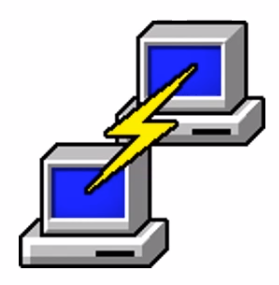
\includegraphics[scale=.15]{imagenes/1_putty.png}
    \end{figure}
    \vspace{-3 mm}
    \item \textbf{Flash ROM}
    Es una herramienta para idenficar el tipo de flash, leer, escribir, verificar e incluso borrar chips de memoria flash. Está especialmente diseñado para trabajar con memorias flash que alberguen BIOS, EFI, firmware y cualquier otra imagen (binario) en dispositivos programables. Puede usarse con el programador CH341A para volcar el firmware de un dispositivo desde su memoria flash. 
    \begin{figure}[htpb]
    \centering 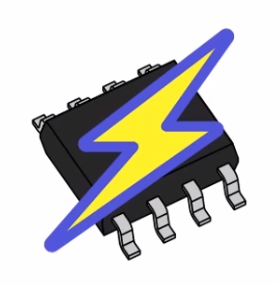
\includegraphics[scale=.15]{imagenes/1_flashrom.png}
    \end{figure}
    \vspace{-3 mm}
    \item \textbf{Binwalk}
    Una vez que obtenemos el firmware, hemos de ser capaces de interrogar al binario (imagen) que hemos descargado para empezar a conocer cosas de ella. Binwalk es una herramienta para buscar archivos empotrados, ejecutables, etc en una imagen de firmware. Ha sido especialmente diseñada para identificar archivos y código embebido en imágenes de firmware. Contiene un archivo con firmas de imágenes que comunmente se encuentran dentro de archivos de firmware, como archivos comprimidos, cabeceras de firmware, kernels de linux, bootloaders, sistemas de archivos, etc.
    \begin{figure}[htpb]
    \centering 
\includegraphics[scale=.15]{imagenes/1_binwalk.png}
    \end{figure}
    \vspace{-3 mm}
    \item \textbf{Ghidra}: Es un framework con utilidades para trabajar con ingeniería inversa. Incluye una suite de herramientas diseñadas para analizar código compilador usando desensamblador, ensamblador, decompilación, scripting etc. Además, Ghidra soporta una amplia variedad de repertorios de instrucciones y de formatos de ejecutables que pueden ser ejecutados tanto en modo interactivo como en modo desatendido (o automático). 
    \begin{figure}[htpb]
    \centering 
\includegraphics[scale=.15]{imagenes/1_ghidra.png}
    \end{figure}
    
    \end{itemize}

\newpage
\subsection{Cómo identificar los pines en UART}

En esta ocasión hemos tenido suerte, pero aún así (no nos esperábamos que ya vinieran marcados) vamos a desarrollar el método usado para identificar qué pines se usan para TX, RX, GND y VCC usando las mediciones de voltage y resistividad que nos proporciona el multimetro. De modo que si damos con un sistema con una interfaz UART y ésta no está marcada (ver figura~\ref{fig:interfazUART}), nuestra primera opción sería consultar el datasheet de la placa, para ver si en ese datasheet identifica a la interfaz UART y además especifica los pines y su identidad. Pero si esta opción tampoco está disponible, entonces nos veremos obligados a realizar mediciones y en base a estas deducir a qué se dedica cada pin. 
 \begin{figure}[htpb]
     \caption{Interfaz UART: así son.}
     \centering
     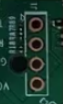
\includegraphics[scale=1]{imagenes/1_UART.png}
     \label{fig:interfazUART}
 \end{figure}

En este esquema básico de mediciones, tenemos tres tipos de mediciones para cada pin. La primera medida será la de la resistencia entre cada pin y tierra (gnd). De esta forma podremos idenficar qué pin es GND. Pues será el pin cuya resistencia sea cero. La segunda medida, mide la resistencia entre cada pin y vcc, así determinaremos qué pin es vcc (el que tenga resistencia cero). El siguiente paso es medir el voltaje en los pines para tratar de identificar quien es TX y quien es RX. 

\begin{table}[htpb]
\centering
\caption{Mediciones eléctricas UART.}
\label{tab:my-table}
\begin{tabular}{@{}clll@{}}
\toprule
{\color[HTML]{FE0000} \textbf{Pin}} & \multicolumn{1}{c}{{\color[HTML]{FE0000} \textbf{R$_{GND}$}}} & \multicolumn{1}{c}{{\color[HTML]{FE0000} \textbf{R$_{VCC}$}}} & \multicolumn{1}{c}{{\color[HTML]{FE0000} \textbf{V}}} \\ \midrule
\multicolumn{1}{|c|}{\textbf{1}}    &                                                               &                                                               &                                                       \\ \midrule
\multicolumn{1}{|c|}{\textbf{2}}    &                                                               &                                                               &                                                       \\ \midrule
\multicolumn{1}{|c|}{\textbf{3}}    &                                                               &                                                               &                                                       \\ \midrule
\multicolumn{1}{|c|}{\textbf{4}}    &                                                               &                                                               &                                                       \\ \bottomrule
\end{tabular}
\end{table}

 Para esto, la sonda negra la vamos a colocar en un lugar que tenga tierra (ver figura~\ref{fig:interfazUARTmediciones}, cerca del botón de reset porque es un trozo de metal que sirve de referencia): 

  \begin{figure}[htpb]
     \caption{Interfaz UART: mediciones gnd.}
     \centering
     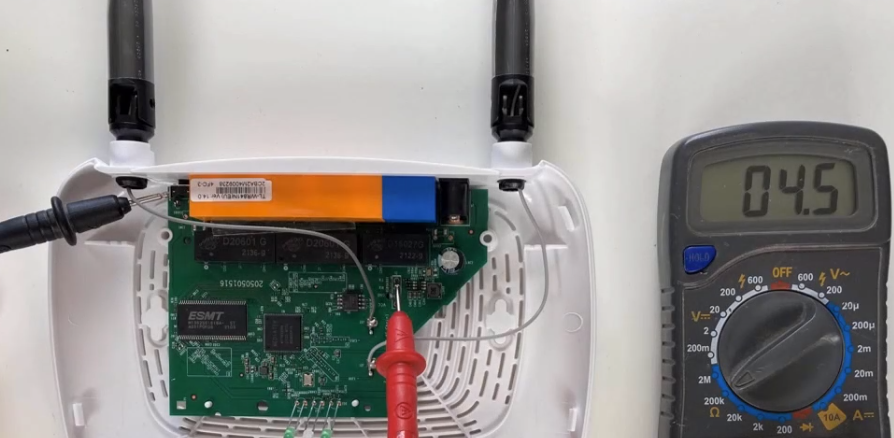
\includegraphics[scale=.4]{imagenes/1_UARTmediciones.png}
     \label{fig:interfazUARTmediciones}
 \end{figure}

La sonda roja está emplazada en el primer pin de la interfaz UART (el más cercano al banco de conexiones ethernet). El multimétro está situado en la medida de resistividad (200K$\Omega$) y la medida nos da \textbf{\textcolor{red}{\emph{0.45k$\Omega$}}}. Si repetimos la operación con el siguiente pin, la medida nos da \textbf{\textcolor{red}{\emph{0.9k$\Omega$}}}, eñ siguiente pin, repitiendo la medición arroja un valor de \textbf{\textcolor{red}{\emph{0.0k$\Omega$}}} de modo que este pin es un candidato perfecto para considerarlo como \textbf{GND} ya que no hay resistencia entre el pin 3 y la medición de la sonda negra (que es el punto que hemos localizado como tierra). El último pin nos da una medición de \textbf{\textcolor{red}{\emph{21.6k$\Omega$}}}. La tabla de mediciones nos queda de esta manera: 


\begin{table}[htpb]
\centering
\caption{Mediciones eléctricas UART: GND}
\label{tab:gnd}
\begin{tabular}{@{}cccc@{}}
\toprule
{\color[HTML]{FE0000} \textbf{Pin}} & {\color[HTML]{FE0000} \textbf{R$_{GND}$}} & {\color[HTML]{FE0000} \textbf{R$_{VCC}$}} & {\color[HTML]{FE0000} \textbf{V}} \\ \midrule
\multicolumn{1}{|c|}{\textbf{1}}    & 4.5 k$\Omega$                             &                                           &                                   \\ \midrule
\multicolumn{1}{|c|}{\textbf{2}}    & 0.9 k$\Omega$                             &                                           &                                   \\ \midrule
\multicolumn{1}{|c|}{\textbf{3}}    & 0.0 k$\Omega$                             &                                           &                                   \\ \midrule
\multicolumn{1}{|c|}{\textbf{4}}    & 21.6 k$\Omega$                            &                                           &                                   \\ \bottomrule
\end{tabular}
\end{table}

Para el siguiente bloque de medidas, como ahora vamos a buscar la diferencia de resistencia entre los pines del UART (para localizar cual es el VCC) lo que hemos de hacer es colocar la sonda negra en un punto de referencia de VCC. Para ellos vamos a usar como referencia el chip de memoria flash, ya que en la hoja de especificaciones del chip indica cual de sus patillas es la patilla VCC (\textcolor{red}{el pin 8 es el pin que se conecta a vcc)}. La figura~\ref{fig:interfazUARTmedicionesvcc} muestra dónde se ha colocado la sonda negra: 

 \begin{figure}[htpb]
     \caption{Interfaz UART: mediciones vcc.}
     \centering
     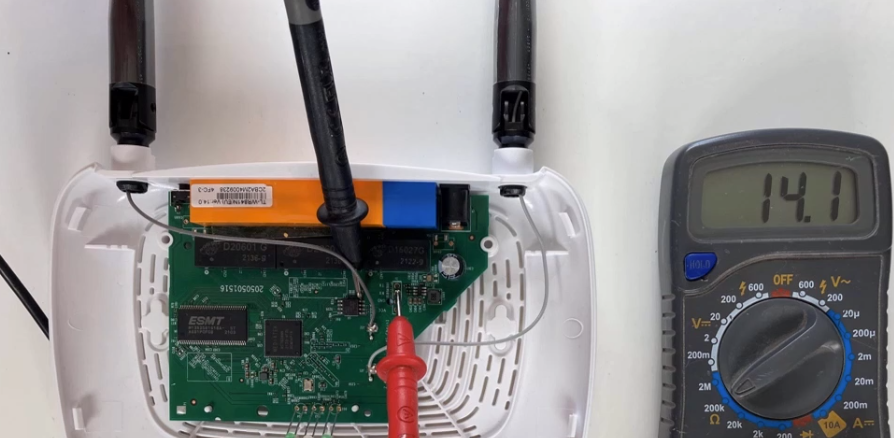
\includegraphics[scale=.4]{imagenes/1_UART_vcc.png}
     \label{fig:interfazUARTmedicionesvcc}
 \end{figure}

Tras mover la sonda roja desde el pin1 hasta el pin4 obtenemos estos valores de resistencias: 

\begin{table}[htpb]
\centering
\caption{Mediciones eléctricas UART: GNDy VCC}
\label{tab:my-table}
\begin{tabular}{@{}cccc@{}}
\toprule
{\color[HTML]{FE0000} \textbf{Pin}} & {\color[HTML]{FE0000} \textbf{R$_{GND}$}}                 & {\color[HTML]{FE0000} \textbf{R$_{VCC}$}}                 & {\color[HTML]{FE0000} \textbf{V}} \\ \midrule
\multicolumn{1}{|c|}{\textbf{1}}    & \multicolumn{1}{c|}{4.5 k$\Omega$}                        & \multicolumn{1}{c|}{14.1 k$\Omega$}                       &                                   \\ \midrule
\multicolumn{1}{|c|}{\textbf{2}}    & \multicolumn{1}{c|}{0.9 k$\Omega$}                        & \multicolumn{1}{c|}{11.0 k$\Omega$}                       &                                   \\ \midrule
\multicolumn{1}{|c|}{\textbf{3}}    & \multicolumn{1}{c|}{{\color[HTML]{FE0000} 0.0 k$\Omega$}} & \multicolumn{1}{c|}{10.0 k$\Omega$}                       &                                   \\ \midrule
\multicolumn{1}{|c|}{\textbf{4}}    & \multicolumn{1}{c|}{21.6 k$\Omega$}                       & \multicolumn{1}{c|}{{\color[HTML]{FE0000} 0.0 k$\Omega$}} &                                   \\ \bottomrule
\end{tabular}
\end{table}


\begin{tcolorbox}[enhanced, title=ATENCION, colback=red!10]
Para el conjunto final de medidas, \textbf{\textcolor{red}{ahora necesitamos conectar la alimentación al router}}. Volvemos a colocar la sonda negra en la referencia de tierra que teniamos localizada. Ojo, al haber conectado la corriente ahora, el router va a registrar actividad en los pines TX y RX. ¿Cual es TX y cual es RX?
\end{tcolorbox}

Una vez que se emplaza la sonda negra en GND, y tenemos alimentado el sistema, sabemos que va a haber actividad entre el chip de flash (firmware) y la memoria SDRAM para cargarlo todo ahí. Para localizar la actividad que tiene cada pin, vamos a usar la sonda roja para averiguar qué valor tiene cada uno, desde el pin1 al pin4. Tras hacer esto, las medidas son :

\begin{table}[htpb]
\centering
\caption{Mediciones eléctricas UART: GND, VCC y TX RX}
\label{tab:my-table}
\begin{tabular}{@{}cccc@{}}
\toprule
{\color[HTML]{FE0000} \textbf{Pin}} & {\color[HTML]{FE0000} \textbf{R$_{GND}$}}                 & {\color[HTML]{FE0000} \textbf{R$_{VCC}$}}                 & {\color[HTML]{FE0000} \textbf{V}} \\ \midrule
\multicolumn{1}{|c|}{\textbf{1}}    & \multicolumn{1}{c|}{4.5 k$\Omega$}                        & \multicolumn{1}{c|}{14.1 k$\Omega$}                       & \multicolumn{1}{c|}{3.25 v}       \\ \midrule
\multicolumn{1}{|c|}{\textbf{2}}    & \multicolumn{1}{c|}{0.9 k$\Omega$}                        & \multicolumn{1}{c|}{11.0 k$\Omega$}                       & \multicolumn{1}{c|}{0.0 v}        \\ \midrule
\multicolumn{1}{|c|}{\textbf{3}}    & \multicolumn{1}{c|}{{\color[HTML]{FE0000} 0.0 k$\Omega$}} & \multicolumn{1}{c|}{10.0 k$\Omega$}                       & \multicolumn{1}{c|}{0.0 v}        \\ \midrule
\multicolumn{1}{|c|}{\textbf{4}}    & \multicolumn{1}{c|}{21.6 k$\Omega$}                       & \multicolumn{1}{c|}{{\color[HTML]{FE0000} 0.0 k$\Omega$}} & \multicolumn{1}{c|}{3.3 v}        \\ \bottomrule
\end{tabular}
\end{table}

El pin 1 ha arrojado valor de resistencia con respecto a GND y VCC, de modo que debe ser o TX o RX. También hemos notado que al conectar la alimentación, este pin 1 ha obtenido valor de voltaje de 3.3 voltios. Y está claro que nadie está enviado nada al dispositivo. De este modo podemos concluir que el PIN 1 es el PIN TX. Si monitorizamos (con el monitor analógico) este pin al alimentar el router podremos comprobar cómo varía el voltaje de este pin rápidamente ya que se está enviando información desde el router hacia el pin TX. Igual que el PIN 1, el PIN 2 muestra resistencia entre GND y VCC. Como el voltaje medido tras alimentar el sistema es cero, parece que éste pueda ser el pin RX ya que nadie está enviando nada al router. PIN 3 es GND ya que no había resistencia con GND (y además, al alimentar el router no tenía voltaje) y PIN 4 es VCC porque no hay resistencia con VCC. 

\begin{table}[htpb]
\centering
\caption{Mediciones eléctricas UART: identidad de los pines}
\label{tab:my-table}
\begin{tabular}{@{}ccccc@{}}
\toprule
{\color[HTML]{FE0000} \textbf{Pin}} & {\color[HTML]{FE0000} \textbf{R$_{GND}$}}                 & {\color[HTML]{FE0000} \textbf{R$_{VCC}$}}                 & {\color[HTML]{FE0000} \textbf{V}} & \multicolumn{1}{l}{{\color[HTML]{3166FF} \textbf{Identidad}}} \\ \midrule
\multicolumn{1}{|c|}{\textbf{1}}    & \multicolumn{1}{c|}{4.5 k$\Omega$}                        & \multicolumn{1}{c|}{14.1 k$\Omega$}                       & \multicolumn{1}{c|}{3.25 v}       & \multicolumn{1}{c|}{TX}                                       \\ \midrule
\multicolumn{1}{|c|}{\textbf{2}}    & \multicolumn{1}{c|}{0.9 k$\Omega$}                        & \multicolumn{1}{c|}{11.0 k$\Omega$}                       & \multicolumn{1}{c|}{0.0 v}        & \multicolumn{1}{c|}{RX}                                       \\ \midrule
\multicolumn{1}{|c|}{\textbf{3}}    & \multicolumn{1}{c|}{{\color[HTML]{FE0000} 0.0 k$\Omega$}} & \multicolumn{1}{c|}{10.0 k$\Omega$}                       & \multicolumn{1}{c|}{0.0 v}        & \multicolumn{1}{c|}{GND}                                      \\ \midrule
\multicolumn{1}{|c|}{\textbf{4}}    & \multicolumn{1}{c|}{21.6 k$\Omega$}                       & \multicolumn{1}{c|}{{\color[HTML]{FE0000} 0.0 k$\Omega$}} & \multicolumn{1}{c|}{3.3 v}        & \multicolumn{1}{c|}{Vcc}                                      \\ \bottomrule
\end{tabular}
\end{table}

\section{Acceso al firmware}
Tal y como ya se ha descrito anteriormente, el firmware es un software que se se \emph{esculpe} en el hardware. Es capaz de operar sin necesidad de acceder a APIs, a un Sistema Operativo o a drivers. Proporciona las instrucciones y la guía necesaria para que el dispositivo pueda operar correctamente comunicandose con otros drivers o realizando funciones y tareas básicas. Ser capaz de extraer el firmware de un dispositivo nos da la oportunidad de identificar debilidades y vulnerabilidades que puedan ser explotadas a través de vectores de ataque tradicionales, tales como ataques vía web o a través de protocolos de red. Además, y esto si es crítico, el firmware almacena información sobre la configuración del dispositivo y datos que pueden llegar a ser sensibles como contraseñas y claves de cifrado. 

\subsection{La ruta de menor resistencia}
Un atacante siempre va a escoger el camino más rápido y sencillo para acceder a un sistema. Y por tanto hemos de buscar estos caminos. Por tanto, para analizar el firmware en este router, podriamos pensar en descargarnos el firmware desde internet, en lugar de tratar de acceder ilegalmente al dispositivo y extraerlo. ¿Es necesario extraer el firmware? ¿Por qué no descargarlo de Internet, analizarlo, revelar las vulnerabilidades y aprovecharlas para atacar al dispositivo? Y en efecto, este sería el paso lógico si no podemos conseguir acceso al router. Los fabricantes prorpocionan acceso al firmware (en Internet) sobre todo para que puedas actualizar tu terminal. A veces, incluso, descargar el firmware es interesante porque las nuevas versiones \textbf{suponen versiones que corrigen vulnerabilidades en versiones previas del firmware} por lo que si identificamos las vulnerabilidades e identificamos a dispositivos que tengan estas versiones previas del firmware, \emph{voilá} ya tenemos el vector de ataque listo. También podemos lograr el firmware a través de los puertos de depuración, esto es una tarea muy dolorosa y costosa. Y esto supondría interrumpir el proceso de arranque e intervenir al \emph{bootloader} de manera que podamos ejecutar comandos para volcar el firmware desde memoria a la pantalla y así capturar la salida gracias a los logs de la consola. Pero, recuerda que la informacón se transifere bit a bit :

\begin{verbatim}
    LAS MATEMÁTICAS NOS ACONSEJAN NO HACERLO: 
    ----------------------------------------
    Tamaño de la memoria flash : 128 Mb
    El firmware, a través de un enlace serie, se vuelca en hexadecimal.
    --> 1 byte = 2 caracteres hexadecimales + 1 espacio
    Cada página de 2 Kb son 64 bytes para corrección de errores.
    --> 3% de sobrecarga del código.
    Un chip de 128 MB = 128 x 3 x 1.03 = 400MB aprox.
    Velocidad del enlace serie = 115.200 kbps = 0.011 Mb/s.
    TIEMPO TOTAL EN DESCARGAR EL FIRMWARE : 9.6 horas.
\end{verbatim}

De modo que para descargar el firmware a través de un enlace serie, tardariamos cerca de \textbf{\textcolor{red}{10 horas}} y no habriamos terminado. Tendriamos un fichero hexadecimal que tenemos que convertir a binario. Truncando todas las cadenas innecesarias. Este sería un método a usar en caso de no tener otro método. 

El próximo método a usar sería el tratar acceder al chip de memoria flash y volcar su contenido.  Para hacer esto podemos conectar el programador CH341A al chip de memoria usando una pinza SOIC y una vez hecho esto tendríamos que lanzar el software \textbf{flashrom} u otro programa similar para extraer el firmware directamente desde memoria. Existe otro método para probar y es intentar conectarse al dispositivo vía TFTP y tratar de conseguir un volcado de memoria a través de este medio, necesitariamos interrumpir el proceso de arranque del router para acceder al \emph{bootloader}; además necesitamos disponer de un servidor TFPT al que conectar el dispositivo que estamos analizando, el servidor TFTP y el dispositivo han de residir en la misma subred. Para esto es necesario que el dispositivo tenga el TFTP activo pero esto es algo muy común porque estos servidores TFTP se usan para actualizar el firmware de los dispositivos, por tanto es muy probable que el dispositivo ya tenga uno. 


Si ninguno de estos métodos funciona, existen otras opciones. Por ejemplo, los dispositivos IoT lanzan una baliza ocasionalmente a los servidores de actualizaciones para comprobar (o reclamar) si hay actualizaciones. En ese caso, usando wireshark (o tcpdump), podemos extraer los paquetes de la actualización. 

\subsection{Conexión vía UART}

El esquema de conexión a la interfaz serie UART del router, conecta el pin TX del router con el pint RX del FT232. El pin TX del FT232 al pin RX del router. Y el pin GND del router con el pin GND del FT232.

 \begin{figure}[htpb]
     \caption{Extracción del firmware a través de la interfaz UART.}
     \centering
     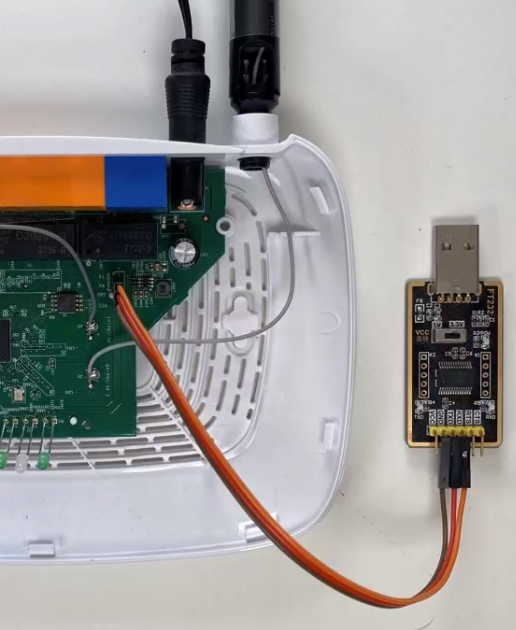
\includegraphics[scale=.4]{imagenes/2_Extraccion_UART.png}
     \label{fig:extraccionUART}
 \end{figure}

Desde Fedora (como es mi caso) o desde Windows, lanzas PuTTY. 
 
 \begin{figure}[htpb]
     \caption{Extracción del firmware a través de la interfaz UART.}
     \centering
     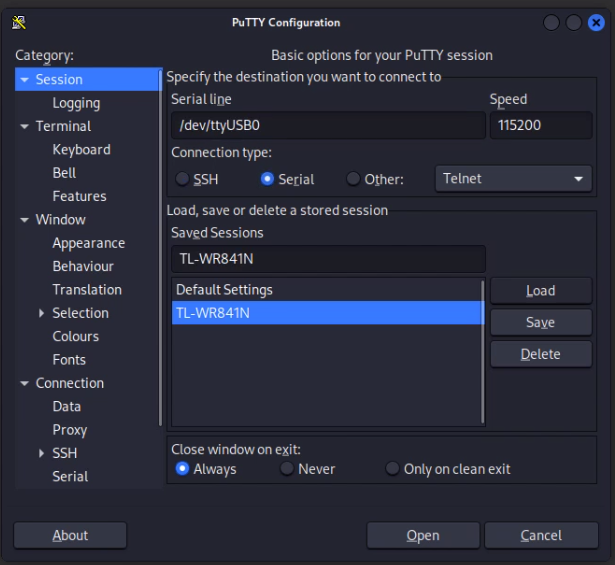
\includegraphics[scale=.4]{imagenes/2_PuTTY.png}
     \label{fig:PuTTY}
 \end{figure}

 Tal como se indica en la figura~\ref{fig:PuTTY}, se deben configurar los parámteros de la conexión (en este caso es serie). El dispositivo (en Linux) en el que se ha mapeado el FT232 es \textbf{\textcolor{red}{/dev/ttyUSBO}}) y la velocidad de transmisión es de 115200 KBps (velocidad de la interfaz UART en el router). En la interfaz de PuTTY, en Session y dentro de Session en la opción Logging seleccionaremos las opciones:
 \begin{itemize}
     \item All session output.
     \item En Log file name consignaremos el nombre del archivo donde queremos guardar los logs de la sesión
     \item Always overwrite it
     \item Flush log file frequently
     \item Include header
     \item Omit known password fields
 \end{itemize}

Hecho esto, tenemos a PuTTY esperando datos desde el UART del router. Una vez que lo encendamos, veremos todo el proceso de arranque del router (figura~\ref{fig:UBOOT}): 

 \begin{figure}[htpb]
     \caption{Proceso de inicio del router vía U-BOOT.}
     \centering
     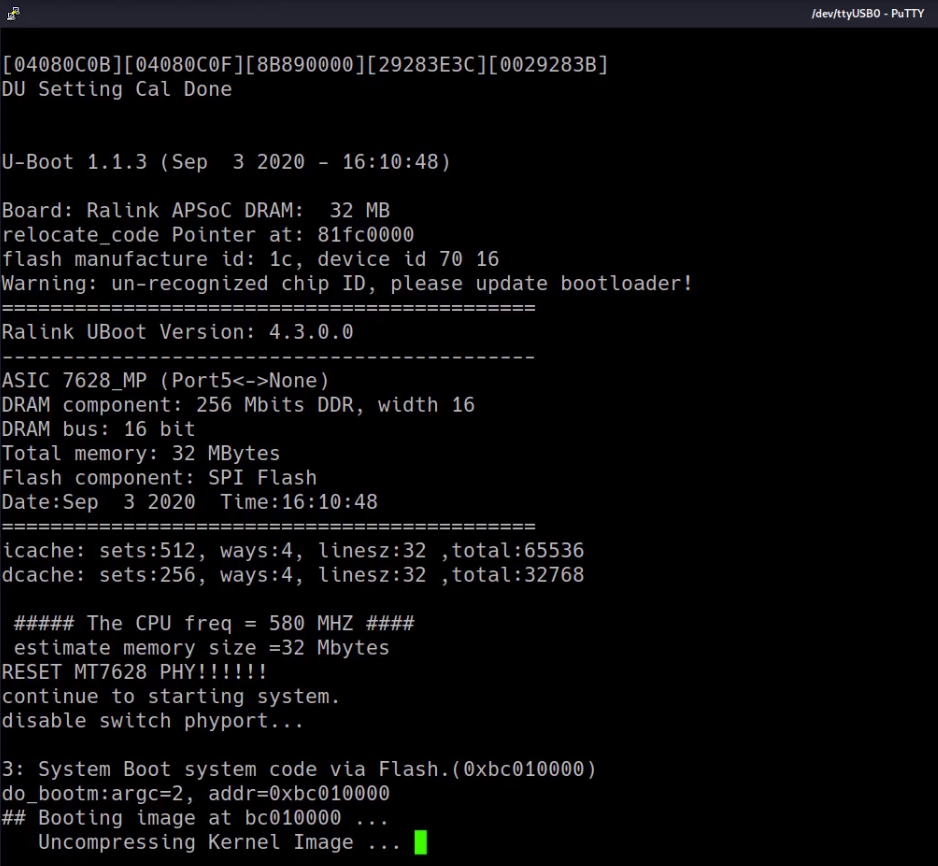
\includegraphics[scale=.4]{imagenes/2_UBOOT.png}
     \label{fig:UBOOT}
 \end{figure}

Hay mucha información interesante y útil en estos mensajes de U-BOOT. Los podremos revisar en nuestro archivo de log. Esta información es interesante porque nos brinda información sobre la organización de la memoria y la localización de los \emph{sistemas de archivos} en memoria. En cuanto que se termina el proceso de inicio del router, a través de la consola serie, obtenemos un prompt. En el inicio del router, hay un proceso que nos genera muchísima información (en el log) que no nos sirve ya que es información de depuración. He localizado el proceso y tan pronto obtenemos el prompt le pedimos al sistema que cierre ese proceso. El proceso tiene el pid=\emph{174} el comando apropiado para que éste proceso de depuración no nos contamine en exceso el archivo de log es: \emph{\textcolor{red}{kill -9 174}} (ver figura~\ref{fig:terminalRouter}). Lo que podemos ver a traves de esta interfaz es similar a lo que veriamos en una consola de un sistema operativo linux convencional:

 \begin{figure}[htpb]
     \caption{Consola del router, accedida vía interfaz serie.}
     \centering
     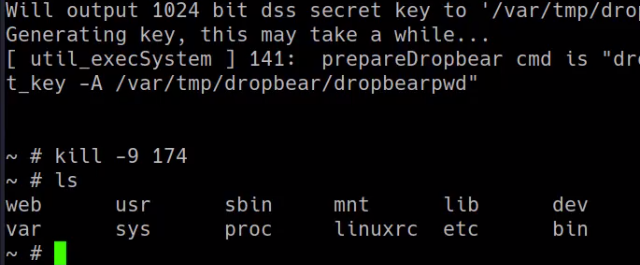
\includegraphics[scale=.6]{imagenes/2_terminalRouter.png}
     \label{fig:terminalRouter}
 \end{figure}

Si listamos el contenido del directorio \emph{bin} (\emph{ls /bin}) podremos comprobar que tenemos disponible a \underline{busybox} que nos permitirá acceder a muchos más comandos de los que nos está ofreciendo la shell del router. Tal como se puede comprobar en la figura~\ref{fig:TFTP}, contamos con el comando TFTP. 

 \begin{figure}[htpb]
     \caption{Entre otros comandos, en busybox, tenemos TFTP.}
     \centering
     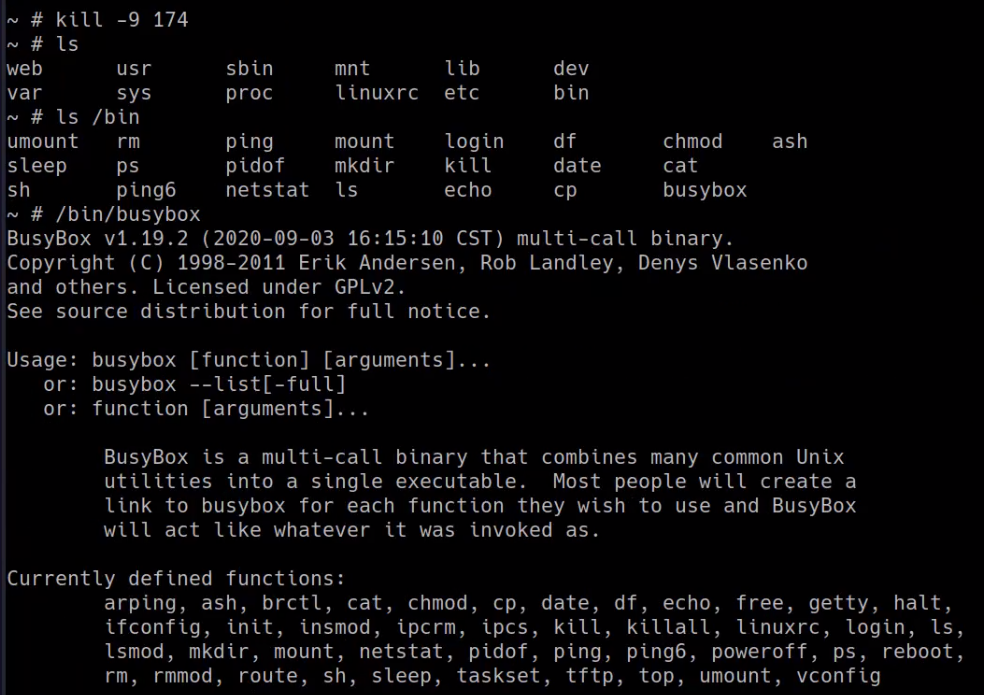
\includegraphics[scale=.4]{imagenes/2_tftp.png}
     \label{fig:TFTP}
 \end{figure}

No obstante, no es una instalación completa de busybox. Si comprobamos el directorio /sbin (sólo se tiene acceso a él si tienes privilegios de super usuario o perteneces al grupo wheel), podemos ver los comandos que tenemos a nuestra disposición: 

\begin{figure}[htpb]
     \caption{Contenido de /sbin y /etc. Listado del fichero /etc/passwd}
     \centering
     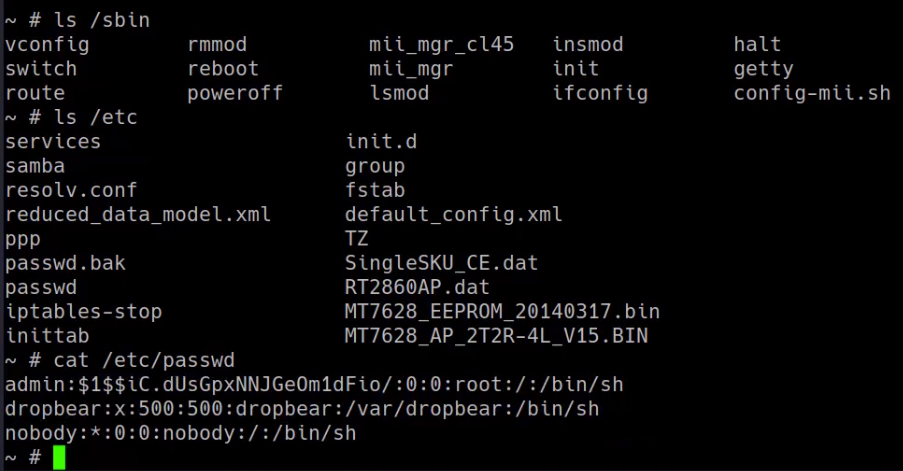
\includegraphics[scale=.4]{imagenes/2_etcsbin.png}
     \label{fig:etcsbin}
 \end{figure}

La figura~\ref{fig:etcsbin} muestra además del directorio /sbin el directorio /etc. En este directorio tenemos el fichero de contraseñas (concretamente el fichero de \emph{hashes de las contraseñas} pero es interesante ver qué usuarios tiene configurado el router. Para el usuario \textbf{admin} podemos ver el hash (que codifica la contraseña) y podríamos usar \textbf{hashcat} para tratar de romper el hash y obtener directamente las credenciales de administración. Pero en este caso, el router es nuestro y no tiene sentido. Lo que nos interesa es conocer qué usuarios tiene para averiguar qué funcionalidad podemos explotar. 

Echar un vistazo al directorio /lib es interesante porque vemos qué funcionalidad está compartida. Un fichero \emph{.so} es una librería que reside en un área en memoria y que es compartida por aquellos programas que precisan usar su funcionalidad, en lugar de incorporar la librería en el espacio de direcciones del programa. De este modo podemos investigar las librerías compartidas que usan lo programas del router y analizar si tienen alguna vulnerabilidad conocida, para así aprovecharla y atacar a aquellos procesos que hagan uso de la librería en cuestión. 

\begin{figure}[htpb]
     \caption{Contenido de /lib}
     \centering
     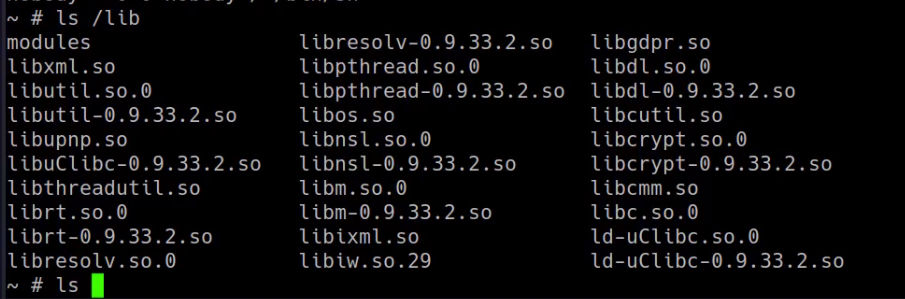
\includegraphics[scale=.4]{imagenes/2_lib.png}
     \label{fig:lib}
 \end{figure}

 De este modo, el siguiente paso (casi) lógico es ver qué procesos se están ejecutando en el router. Para esto lanzamos un \emph{ps}, lo que nos da información muy interesante: 

 \begin{figure}[htpb]
     \caption{Procesos en ejecución: interesante ver httpd y dropbear.}
     \centering
     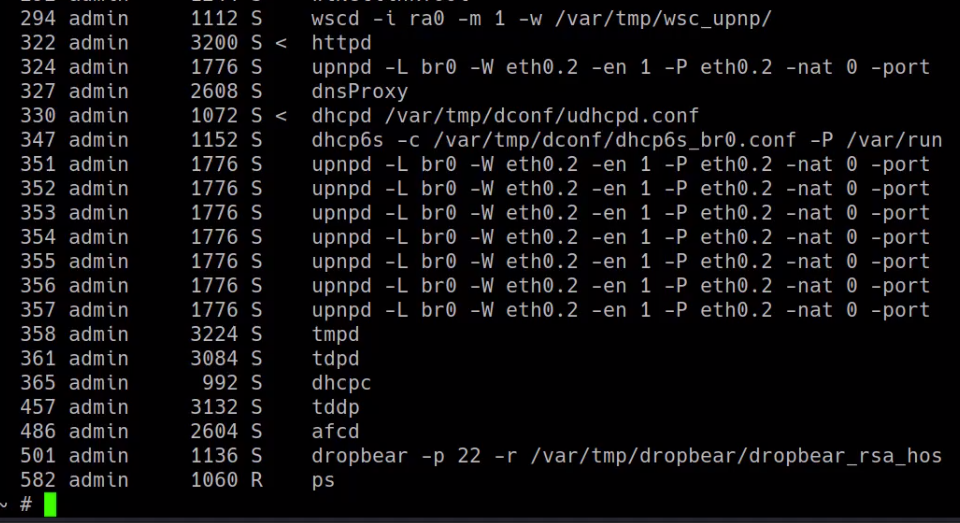
\includegraphics[scale=.4]{imagenes/2_httpdssh.png}
     \label{fig:httpddropbear}
 \end{figure}

 Vemos que tenemos al \textcolor{red}{servidor SSH dropbear} en el puerto \textcolor{red}{22} y vemos que tenemos un \textcolor{red}{daemon http}, por lo que tenemos un servidor web en el router. Este servidor web se usa para ofrecer al usuario una interfaz de configuración. La figura~\ref{fig:netstat} muestra cómo, con el comando \emph{netstat} podemos ver qué conexiones tiene el router abiertas. No está conectado a Internet, recordemos esto. 

  \begin{figure}[htpb]
     \caption{Conexiones abiertas (netstat).}
     \centering
     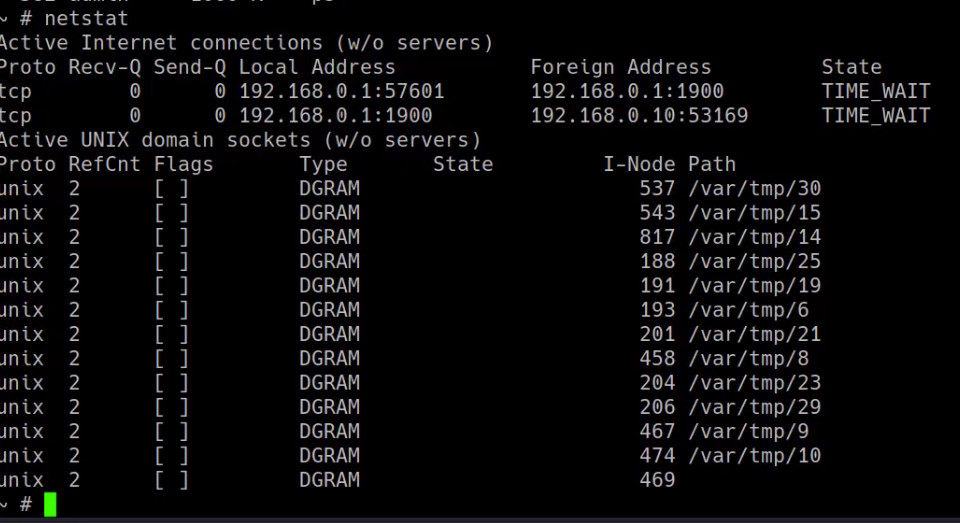
\includegraphics[scale=.4]{imagenes/2_netstat.png}
     \label{fig:netstat}
 \end{figure}

 En esta figura~\ref{fig:netstat} los puertos 21 (FTP) y 23 (TELNET) son interesantes y reveladores. Nuestro router abre esas puertas. Ya tenemos una idea aproximada de la configuración básica del router, lo siguiente es comprobar hasta dónde (qué privilegios) puedo llegar en el router. Para esto hemos de comprobar como qué usuario estoy logueado en el sistema. Recordemos, viendo el fichero /etc/passwd que había tres usuarios, el comando \emph{whoami} me dará información sobre el usuario que estoy usando vía UART. Desafortunadamente no disponemos de ese comando. Tampoco disponemos de \emph{uname} que me permitiría ver detalles del kernel usado. 

 En esta situación, nos queda usar \emph{busybox} y TFTP, una opción sería ampliar los comandos disponibles usando TFTP para descargar una versión más avanzada y completa de busybox. Si disponemos de más comandos podremos obtener más información. No obstante, si seguimos tratando de obtener más información del sistema, en este caso del sistema de archivos usado y dónde podemos escribir (descargar cosas). Para esto podemos usar el comando \emph{mount}. Esto nos indica que la única parte del sistema de archivos donde puedo escribir (¡exacto! para descargar un busybox más completo) es /var. 
 
  \begin{figure}[htpb]
     \caption{¿Dónde podemos desplegar cosas (escribir)?.}
     \centering
     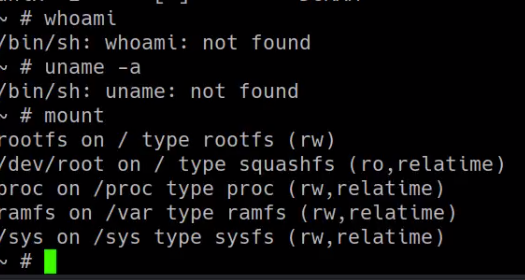
\includegraphics[scale=.4]{imagenes/2_var.png}
     \label{fig:var}
 \end{figure}

\begin{tcolorbox}[colback=red!10, title=Motamos nuestro servidor TFTP]
    Tenemos que preparar nuestro \textbf{payload}. En este caso será una versión de busybox para MIPS (\emph{busybox-mipsel}). Para esto tenemos que descargar el fichero desde este servidor web: \href{https://busybox.net/downloads/binaries/1.16.1/}{https://busybox.net/downloads/binaries/1.16.1/} y seleccionar el fichero \emph{busybox-mipsel}. 

    Los pasos seguidos serían: 
    \begin{itemize}
    \item \textbf{SUBRED:} Conectar el portátil al router, para que tengan la misma subred (la dirección IP que se le asigna a mi portátil es 192.168.0.10).
    \item \textbf{TFTP:} Instalar un servidor de TFTP y dejar en el directorio raiz el fichero descargado que nos proporciona un busybox más potente.
    \item \textbf{Conexión al servidor desde el router}: Pretendemos descargar el fichero \emph{busybox-mipsel} en el directorio /var del router. Para esto tenemos que, desde el router, ejecutar el comando: 
    \begin{itemize}
        \item \textbf{cd /var} (acceso al directorio var, que es el único en el que podemos escribir).
        \item \textbf{tftp -g -r busybox-mipsel 192.168.0.10} (los parametros usados son g: get y r: remote). 
    \end{itemize}
    \item \textbf{Descargado:} lo tenemos que hacer ejecutable, para eso ejecutamos \textbf{chmod +x busybox-mipsel}.
    \end{itemize}
\end{tcolorbox}

Una vez que ya tenemos dentro del router nuestro \emph{busybox-mipsel} ya podemos ejecutarlo con \emph{./busybox-mipsel} (desde dentro del directorio /var que es donde lo hemos descargado, claro). Y podemos ver tres cosas (ver figura~\ref{fig:busyboxgrande}):
\begin{itemize}
    \item Al ejecutar \emph{./busybox-mipsel} vemos que la cantidad de comandos disponibles es mucho mayor que con el \emph{busybox} que traer el router por defecto.
    \item Ahora podemos ejecutar \textbf{whoami} para ver qué usuario se me asigna. El usuario es \textbf{admin}.
    \item Ahora podemos ver los detalles del kernel (2.6.36) sobre una arquitectura mips. Me llama la atención que un router comprado en 2023 tenga un kernel de 2010. Al ser tan viejo seguro que hay varias vulnerabilidades que podemos aprovechar.
\end{itemize}

  \begin{figure}[htpb]
     \caption{Busybox-mipsel: acceso a más comandos.}
     \centering
     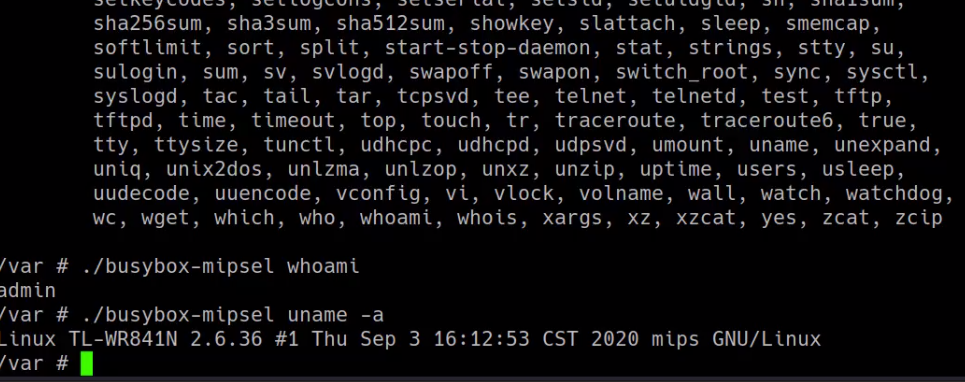
\includegraphics[scale=.4]{imagenes/2_busyboxgrande.png}
     \label{fig:busyboxgrande}
 \end{figure}

 Llegados a este punto, he descubierto que el router (si entro por la interfaz serie (UART)) me da acceso de administrador. De modo que la parte más difícil podemos considerarla ya terminada, tenemos acceso \emph{root} al dispositivo. Ahora debemos aprovechar esta circunstancia para extraer el firmware del dispositivo.

\subsubsection{Extracción del firmware a través del UART}
Si revisamos el log, podemos ver que durante el proceso de arranque del router se crean cinco particiones MTD (Memory Technology Device), se usan -en Linux- para interactuar la memoria flash (que es donde está almacenado el firmware). Este subsistema se creó para hacer de intermediario (abstraer) a los drivers especificos hardware de las aplicaciones de más alto nivel. 
  \begin{figure}[htpb]
     \caption{Particiones MTD (Memory Technology Device).}
     \centering
     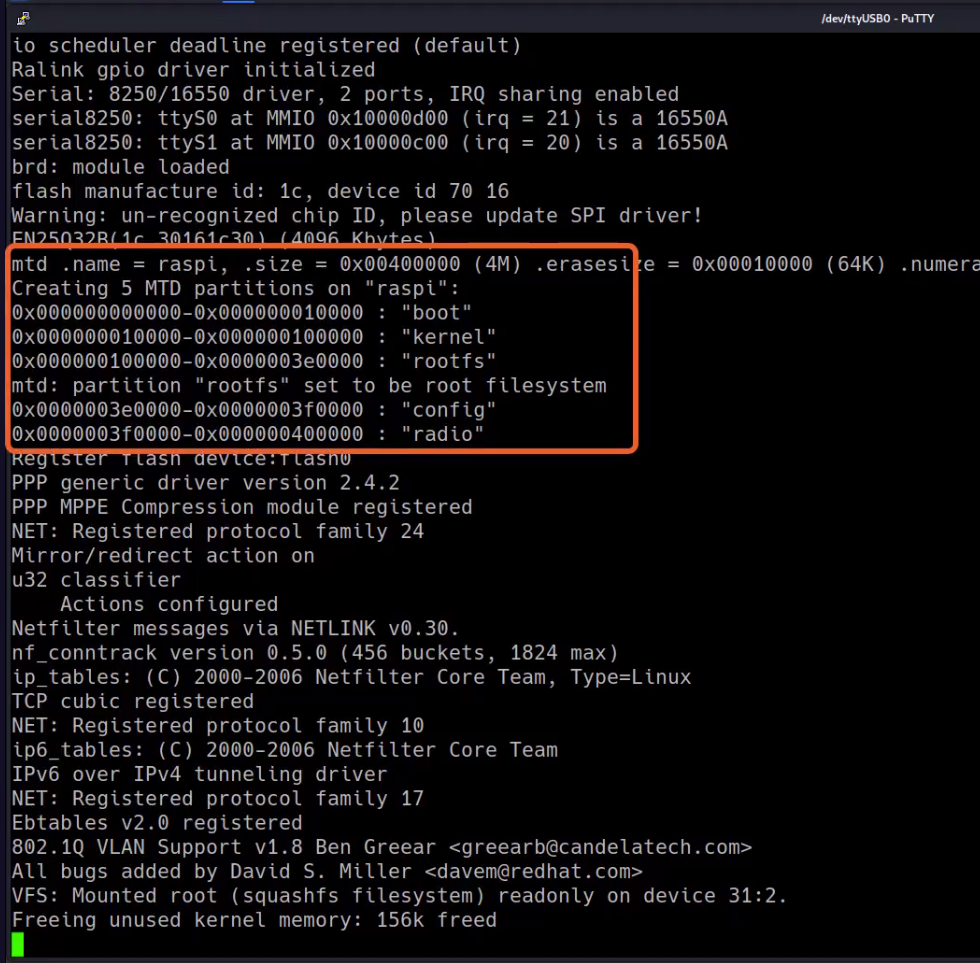
\includegraphics[scale=.4]{imagenes/2_mtd.png}
     \label{fig:mtd}
 \end{figure}

Una vez que estamos dentro del router podemos ver la información de la partición MTD dentro del sistema de archivos virtual en /proc. Este subsistema MTD en /proc se monta dentro del directorio /dev (devices). 

   \begin{figure}[htpb]
     \caption{Particiones MTD (Memory Technology Device) en /proc ).}
     \centering
     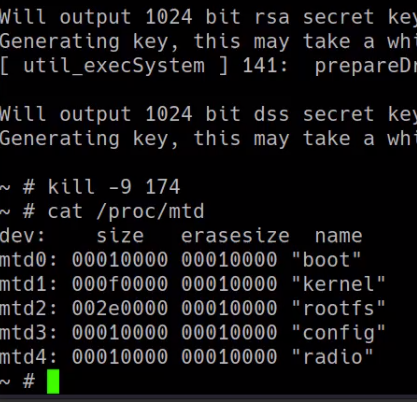
\includegraphics[scale=.6]{imagenes/2_procMTD.png}
     \label{fig:procmtd}
 \end{figure}

De modo que si listamos el contenido del directorio /dev (\emph{ls -al /dev}): 

   \begin{figure}[htpb]
     \caption{Particiones MTD (Memory Technology Device) en /dev.}
     \centering
     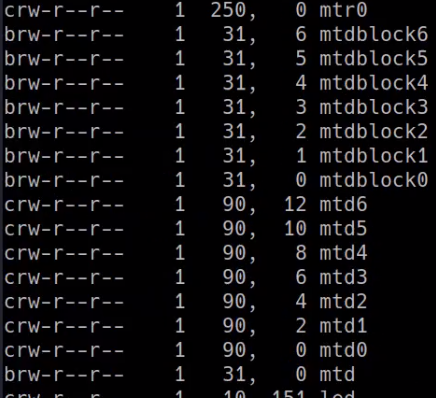
\includegraphics[scale=.6]{imagenes/2_devmtd.png}
     \label{fig:devmtf}
 \end{figure}

 Si observamos los permisos, podemos ver que los bloques MTD desde el cero hasta el seis son dispositivos de bloque\footnote{Son dispositivos de almacenamiento masivo no volatil cuya información puede accederse de manera aleatoria, más especificamente un bloque MTD se usa para presentar la memoria flash como un dispositivo de bloque que puede ser formateado y montado con si fuera parte del sistema de archivos.  }. Si miramos dentro de uno de estos dispositivos ( \emph{cat /dev/mtdblock0} ) veremos una mezcla de caracteres, algunos legibles otros ilegibles. 

    \begin{figure}[htpb]
     \caption{Contenido (caracteres) de un bloque mtd.}
     \centering
     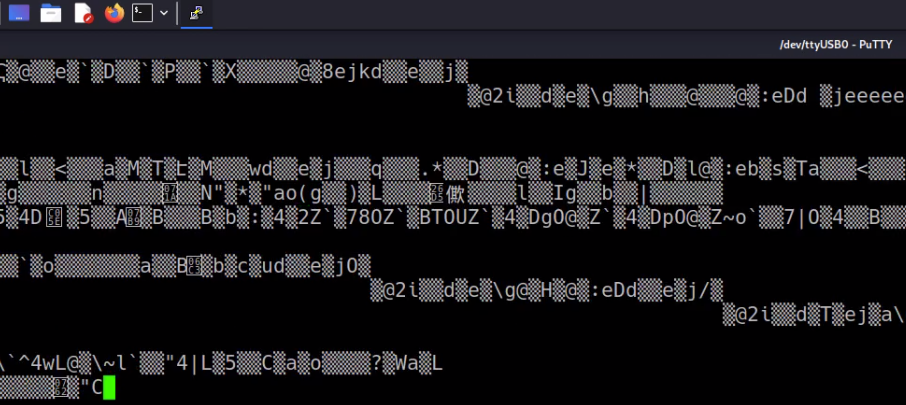
\includegraphics[scale=.4]{imagenes/2_garbage.png}
     \label{fig:garbage}
 \end{figure}

 Por otro lado es lo que esperamos encontrar, igual que cuando abrimos con un editor ascii un disco o una unidad USB. Por tanto, si queremos \emph{acceder al contenido de los MTD} podemos hacerlo con \emph{cat} y guardar su salida, y luego abrirla con \emph{binwalk}. Para hacer esto, en lugar de hacerlo de esta forma, lo vamos a realizar a través del siguiente script python que realiza una conexión serie y extrae el contenido de cada MTD. 

 \begin{tcolorbox}[colback=blue!10, title=Script para acceder al contenido de los MTD: extraccion\_via\_uart.py]
     \begin{verbatim}
import serial
import time

port = serial.Serial("/dev/ttyUSB0", baudrate=115200, timeout=60.0)
port.write("\n".encode())
time.sleep(1)

    while True:
        port.flush()
        time.sleep(1)
        f = open("rootfs_via_uart.img", "w")
        f.write('')
        f.close()
        f = open("rootfs_via_uart.img", "a")
        port.write("cat /dev/mtdblock2\n".encode())

        buffer = ''
        contador = 0
        while True:
            time.sleep(0.001)
            bytesporleer = port.inWaiting()
            time.sleep(0.001)
            contador = contador + 1
            if bytesporleer > 0: 
                contador = 0
                print ("Bytes por leer: " + str(bytesporleer))
                buffer = port.read(bytesporleer)
                print ("Leído: " + str (Buffer))
                f.write(buffer.decode(encoding='latin-1'))
                time.sleep(0.001)
            if contador > 1000:
                if t.tell() > 2000000:
                    print ("Hemos terminado")
                    while True:
                        pass
                print ("Error! Tamaño: " + str(f.tell()) + " Bytes")
                port.write("\x03".encode())
                time.sleep(1)
                break
                    
         
     \end{verbatim}
 \end{tcolorbox}

Si desde el terminal de linux (o consola de windows) lanzamos el script python: \emph{python extraccion\_via\_uart.py} obtendremos en pantalla (porque en el script lo estamos mostrando por pantalla además de meterlo en un fichero, podemos eliminar el verlo por pantalla e irá más rápido): 

\begin{figure}[htpb]
     \caption{Descarga de 496 bytes por iteración vía UART.}
     \centering
     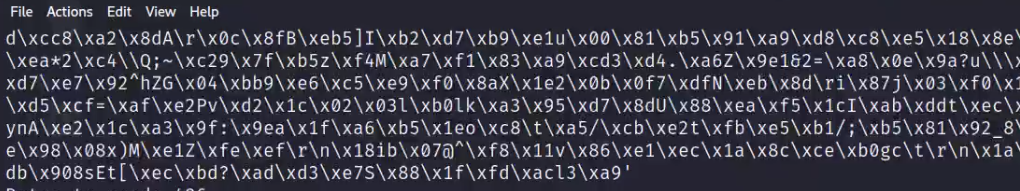
\includegraphics[scale=.4]{imagenes/2_dump.png}
     \label{fig:dump}
 \end{figure}

 La descarga de este archivo ha tomado casi media hora. Antes de poder analizar este binario con \textbf{binwalk} debemos eliminar las cadenas innecesarias y convertir el hexadecimal a binario. Para esto, cualquier conversor de fichero volcado en hexadecimal a binario nos sirve. Al comprobar con el comando \emph{binwalk rootfs\_via\_uart.img} encontramos un sistema de archivos \textbf{squash} de 3 MB. 

 \begin{figure}[htpb]
     \caption{binwalk en el fichero descargado.}
     \centering
     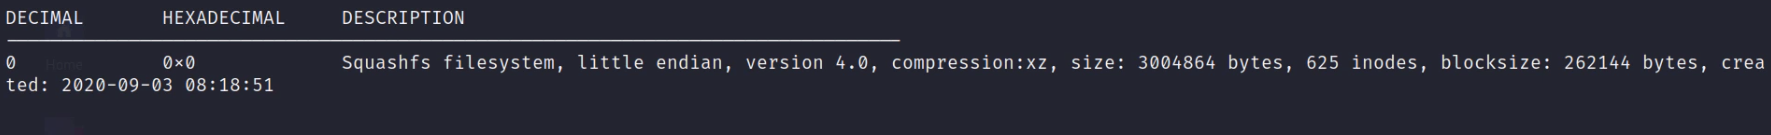
\includegraphics[scale=.28]{imagenes/2_binwalk.png}
     \label{fig:binwalk}
 \end{figure}

\subsection{Extracción vía volcado de la memoria flash}
¿Qué pasa si no podemos tener acceso a una consola (terminal) que nos de acceso a la línea de comandos del router? Pues que tendremos que realizar la extracción atacando directamente el chip que contiene el firmware, esto es el chip de memoria flash utilizando el programador CH341A y la aplicación \textbf{flashrom}. Lo que extraigamos, igual que antes, será verificado usando \emph{binwalk}. 

 \begin{figure}[htpb]
     \caption{Extracción directa desde el chip usando una pinza SOIC y el programador CH341A.}
     \centering
     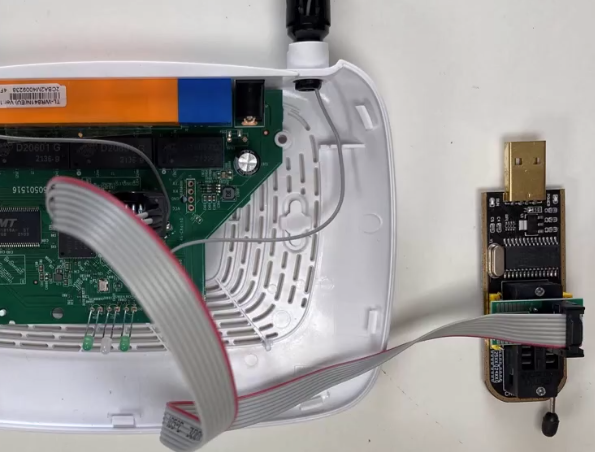
\includegraphics[scale=.5]{imagenes/2_ch341A.png}
     \label{fig:ch341a}
 \end{figure}

En la pinza SOIC, el cable rojo se debe colocar en el pin 1 del chip. El pin 1 suele ser el que está marcado en el chip. Conectarlo es un poco complicado porque a veces la pinza se suelta y debe comprobarse que todo queda bien conectado cuando se vuelva a colocar. Si se usa una pinza que no sea SOIC entonces es probable que sólo se necesiten concetar los pines especificos para la comunicación SPI (estos son 1, 2, 4, 5 y 6 en este chip). Se debe consultar la hoja de especificaciones técnicas para estar seguro de qué pines usar. En este chip los pines van del 1 al 4 (el 1 es el que tiene la marca) y del 5 al 8 en el lado opuesto. 

\begin{tcolorbox}[colback=red!10, title=Atención]
    Para la extracción del firmware desde el chip de memoria flash, no se debe conectar la alimentación pues esto iniciaría el proceso de arranque del router y el chip, que justamente inicia todo es en el que vamos a trabajar ahora.
\end{tcolorbox}

\begin{tcolorbox}[colback=green!10, title=Usar flashrom para leer el chip de memoria flash]
    \textbf{flashrom --programmer ch341a\_spi -r TL-WR841N\_firmware.bin}
    En este caso estamos usando un programador genérico CH341A. La opción -r instruye a flashrom a leer desde la flash y a guardar lo que lea en el archivo que le indiquemos.
    Es frecuente que flashrom solicite escalar a un usuario con privilegios, pero en nuestro caso no es necesario pues estamos usando un programador USB que flashrom soporta.
\end{tcolorbox}

Al ejecutar flashrom, ésta tarda muy poco en identificar la memoria con la que queremos trabajar. Este método ha tardado menos de cuarenta segundos en obtener todo el contenido de la memoria flash. 
 \begin{figure}[htpb]
     \caption{Flashrom.}
     \centering
     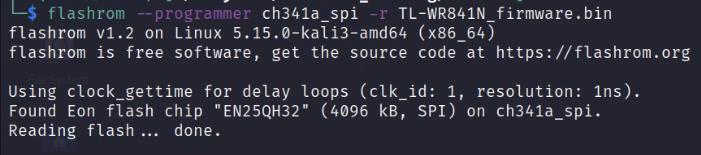
\includegraphics[scale=.7]{imagenes/2_flashrom1.png}
     \label{fig:flashrom1}
 \end{figure}

 En este caso, al contrario que durante la extracción via UART, no es necesario preprocesar el archivo bin porque lo extraemos bit a bit, directamente desde donde está almacenado. Es un método más rápido y menos tedioso. Tras la descarga del firmware, siempre es necesario revisarlo con \textbf{binwalk} de modo que podremos comprobar si las imágenes han sido creadas correctamente o no.

  \begin{figure}[htpb]
     \caption{Binario extraído desde el chip de flash sometido a binwalk}
     \centering
     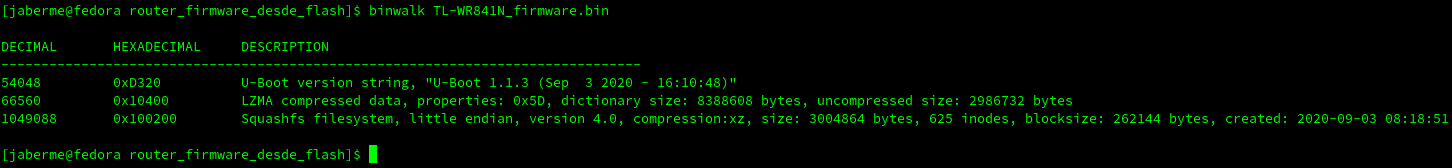
\includegraphics[scale=.35]{imagenes/2_flash.png}
     \label{fig:flash}
 \end{figure}

Rápidamente se puede ver el cargador U-BOOT, información comprimida con el algoritmo LZMA y un sistema de archivos \emph{SquashFS}. Asi que parece que hemos obtenido, de nuevo, correctamente la imagen.

\subsection{Extracción vía TFTP directamente desde la RAM}
 En este método se accede al sistema de archivos desde el MTD. Pero en lugar de extraerlo a través de una conexión serie lenta (como UART) lo haremos a través de TFTP, que ya dejamos instalado cuando isntalamos \emph{busybox-mipsel} en el directorio /var. 

Lo que tenemos que preparar, de nuevo, es nuestro pequeño servidor TFTP que será quien reciba el firmware. De modo que ahora volvemos a conectar el FT232 a los pines UART igual que hicimos en la sección de UART. De este modo vamos a volver a tener acceso a la consola (terminal del router) y si, lo que vamos a hacer es inicar una conexión FTP desde el router a nuestro servidor TFTP y le vamos a enviar el firmware. En esta ocasión vamos a conectar el router con nuestro portátil con un cable de red ethernet. Los dos se configuran para estar en la misma subred. Como vamos a acceder a la RAM y ésta está representada a través de los dispositivos de bloque MTD (ver figura~\ref{fig:mtd}) hemos de recordar que contabamos con cinco particiones que se crean cuando el router se reinicia. La presencia de las particiones se podía comprobar, tal como se vió en la figura~\ref{fig:procmtd} con el comando \emph{cat /proc/mtd}. Podemos extraer cada una de esas particiones, pero la más importante es la partición \textbf{rootfs}. 

  \begin{figure}[htpb]
     \caption{Envío del firmware vía tftp}
     \centering
     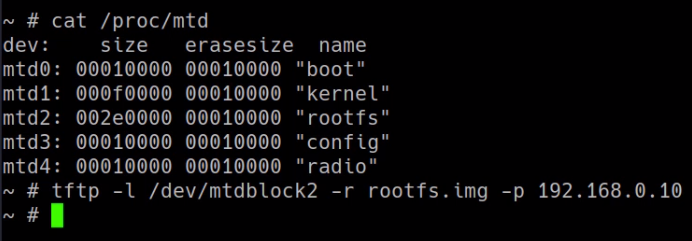
\includegraphics[scale=.35]{imagenes/2_tftpram.png}
     \label{fig:tftpram}
 \end{figure}

 En pocos segundos habremos recibido la partición rootfs en nuestro servidor. 
 
 
\section{Análisis de firmware}

Lo que tenemos ahora en nuestro poder es un fichero binario, la imagen del firmware de nuestro dispositivo objetivo. Con ella podemos realizar varias tareas, que se pueden dividir en dos bloques: 
\begin{itemize}
    \item \textbf{Información Sensible:} Identificar información sensible en la imagen, por ejemplo, credenciales, claves de cifrado, hashes, etc.
    \item \textbf{Búsqueda de vulnerabilidades en el hardware}: Averiguar qué software tiene instalado el router para tratar de buscar sus debilidades. Vulnerabilidades que puedan incluso afectar al propio sistema operativo del dispostivo.
\end{itemize}

Antes de realizar operación alguna hemos de identificar y comprender la estructura de la imagen que hemos obtenido desde el router. La figura~\ref{fig:rom} muestra el fichero raw binario que hemos extraído del router. Como vamos a realizar operaciones sobre él, por precaución, hacemos la copia en rom2.bin para analizar y comprender la estructura del fichero. En esta figura podemos ver que \emph{binwalk} (el comando para analizar es directo : \emph{binwalk rom2.bin} en nuestro caso) es capaz de interpretar la estructura interna del archivo binario. 

  \begin{figure}[htpb]
     \caption{Imágenes extraídas del router}
     \centering
     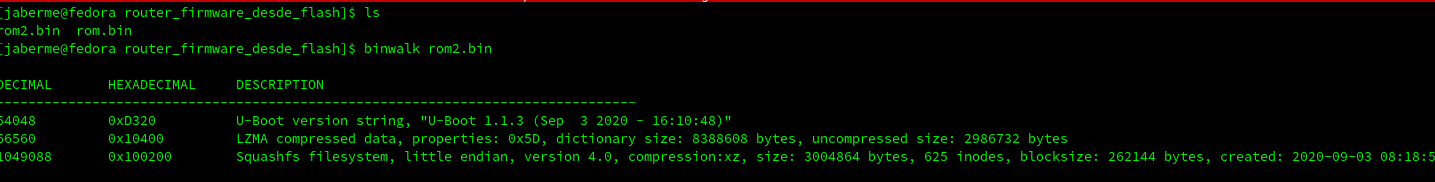
\includegraphics[scale=.35]{imagenes/rom.png}
     \label{fig:rom}
 \end{figure}

El archivo binario que hemos extraído contiene : 
\begin{itemize}
    \item El bootloader que usa el router para arrancar todo (cargar la imagen del sistema operativo en memoria):
    \begin{tcolorbox}[colback=red!10]
            \begin{verbatim}
U-Boot version string, "U-Boot 1.1.3 (Sep  3 2020 - 16:10:48)".
            \end{verbatim}
    \end{tcolorbox}
    Podemos ver que el bootloader comienza en el byte 54048.
    \item Ficheros comprimidos con LZMA
    \begin{tcolorbox}[colback=red!10]
            \begin{verbatim}
LZMA compressed data.
            \end{verbatim}
    \end{tcolorbox}
    Estos datos comienzan a partir del byte 66560. 
    \item El sistema de archivos completo del router. 
    \begin{tcolorbox}[colback=red!10]
            \begin{verbatim}
Squashfs filesystem, little endian, version 4.0.
            \end{verbatim}
    \end{tcolorbox}
    El sistema de archivos comienza alrededor de 1 MB (byte 1049088). 
\end{itemize}

Binwalk a veces da falsos positivos o información errónea. Por ejemplo, en el segmento que corresponde con los datos comprimidos (LZMA) nos indica que el diccionario comprimido ocupa 8.3 MB pero que, por el contrario, descomprimido ocupa 2.9 MB. A parte de esto, binwalk nos permite analizar la \textbf{entropía} del binario. 

\begin{tcolorbox}[colback=green!10]
    La \textbf{entropía} es un concepto heredado de otras disciplinas como la termodinámica o la química. Esta magnitud mide el desorden. Y por tanto la irreversibilidad. Además, en la ingeniería en informática se usa para determinar si por ejemplo un segmento de información binaria está cifrado y por tanto puede contener (en determinados contextos) malware. En un archivo binario, la entropia mide la aleatoriedad de la información. 
\end{tcolorbox}

La figura~\ref{fig:entropia} muestra la aleatoriedad del firmware del router. El eje Y muestra la entropía (valor desde 0 a 1). Los valores de entropía altos (se considera alto por encima de 0.7) suelen indicar que los datos están \textbf{ofuscados\footnote{La ofuscación consiste en añadir información inservible a información útil para dificultar el proceso de análisis}} precisamente porque si sabemos que el fichero contiene información que no es de naturaleza aleatoria (como puede ser un archivo binario que contiene una estructura concreta) y la entropía es alta (es decir, sabemos que no es aleatorio pero la entropía me dice que sí) sólo puede significar que la información útil está tratando de ser escondida (ofuscada). 
\begin{figure}[htpb]
     \caption{Entropía de rom.bin}
     \centering
     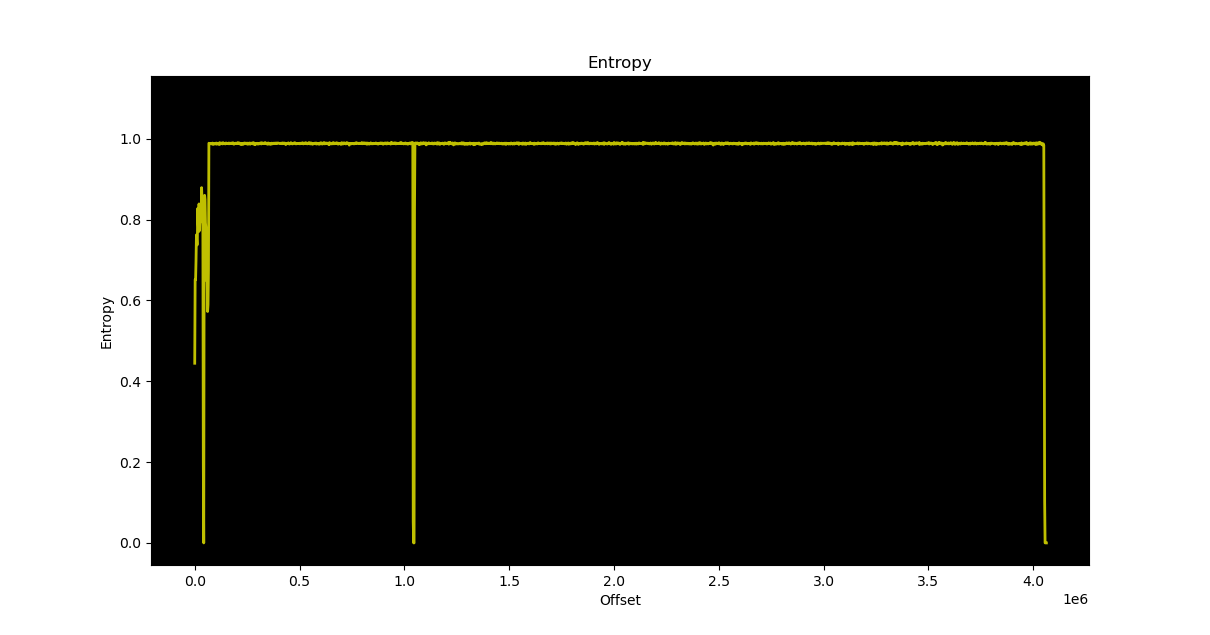
\includegraphics[scale=.6]{imagenes/entropia.png}
  \label{fig:entropia}
\end{figure}
La figura~\ref{fig:entropia} nos indica que la mayor parte del archivo está ofuscada salvo una pequeña parte al princio. De las tres partes que componen el archivo binario, la más interesante para tratar de verificar la seguridad del router es precisamente la última, la que contiene al sistema de archivos \textbf{Squashfs}. 

\begin{tcolorbox}[colback=green!10]
\textbf{Squashfs} es un sistema de archivos Linux \textbf{comprimido} y de solo lectura. Asi que es muy probable que si en un dispositivo (en este caso nuestro router) encontramos un Squashfs lo que tendremos ahí es todo el arbol de directorios. 
\end{tcolorbox}

\subsection{Analizar la parte interesante del binario que acabamos de extraer}
Necesitamos extraer, del archivo binario rom.bin (en nuestro caso, para no quedarnos sin la prueba original extraída del router), el segmento binario que se corresponde con el sistema de archivos squashfs. 

\begin{tcolorbox}[colback=green!10]
Para extraer información podemos usar las capacidades de \textbf{binwalk} aunque también veremos cómo usar el comando Linux \textbf{dd}, es preciso conocer ésta técnica cuando no tengamos la opción de usar binwalk. Podemos usar directamente la opción -e : \textbf{\emph{binwalk -e rom2.bin}}, esto extraerá toda la información del binario. Pero también podemos separar del bianrio los diferentes segmentos (en binario) con el comando: \textbf{\emph{binwalk --dd='.*' rom2.bin}}
\end{tcolorbox}

Si lanzamos el comando \textbf{\emph{binwalk --dd='.*' rom2.bin}}, obtendremos (ver figura~\ref{fig:extraccion1}) varios archivos binarios (entre ellos se puede distinguir el archivo comprimido LZMA. 

\begin{figure}[htpb]
     \caption{Extracción de los binarios de rom.bin}
     \centering
     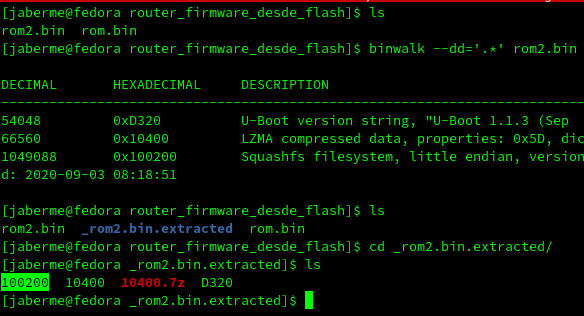
\includegraphics[scale=.6]{imagenes/extraccion1.png}
  \label{fig:extraccion1}
\end{figure}

Si observamos, hay un fichero binario que se llama igual que (en hexadecimal) el byte a partir desde el que comienza el sistema de archivos (100200). Ese archivo, si lo analizamos con binwalk de nuevo, veremos que ahora tenemos aislado al sistema de archivos: 
\begin{figure}[htpb]
     \caption{Extracción de los binarios de rom.bin}
     \centering
     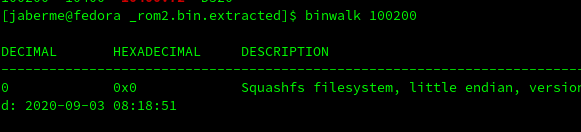
\includegraphics[scale=.6]{imagenes/extraccion2.png}
  \label{fig:extraccion2}
\end{figure}

Ahora ya podemos extraer el contenido usando el comando \textbf{\emph{binwalk -e 100200}}. ¿Podríamos haber ejecutado este comando \textbf{\emph{binwalk -e rom2.bin}} y haber extraído todo lo que había en el binario (bootloader, LZMA y squasfh)? SI. Pero en este caso hemos preferido extraer el binario que nos interesa desde el firmware (rom2.bin) y luego desde ese binario sólo sacar el contenido que guarda dentro. En lugar de extraer todo el contenido de todos los binarios que se guardan en rom2.bin. 

Tras la extracción se crea (en nuestro caso) el directorio \textcolor{blue}{\textbf{\_100200.extracted}} y dentro de ese directorio, tenemos lo que realmente nos interesa que es el \textcolor{blue}{\textbf{squashfs-root}}:

\begin{figure}[htpb]
     \caption{squashfs}
     \centering
     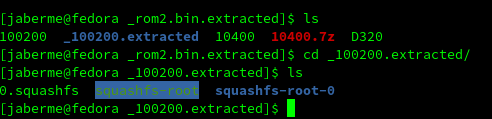
\includegraphics[scale=.6]{imagenes/squashfs-root.png}
  \label{fig:squashfs}
\end{figure}

Si accedemos a este directorios, veremos que tenemos acceso a todo el arbol de directorios. Si entramos en /etc (ver figura) hay dos ficheros muy interesantes

\begin{figure}[htpb]
     \caption{Archivos interesantes en squashfs-root/etc}
     \centering
     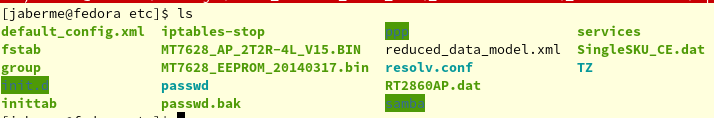
\includegraphics[scale=.6]{imagenes/passback.png}
  \label{fig:pass}
\end{figure}

\begin{itemize}
    \item passwd.bak: si miramos dentro el contenido es justo el que vimos antes:
    \begin{itemize}
        \item admin:\$1\$\$iC.dUsGpxNNJGeOm1dFio/:0:0:root:/:/bin/sh
        \item dropbear:x:500:500:dropbear:/var/dropbear:/bin/sh
        \item nobody:*:0:0:nobody:/:/bin/sh
    \end{itemize}

    \begin{tcolorbox}[colback=blue!10]
       \textbf{Usuarios}: admin:\$1\$\$iC.dUsGpxNNJGeOm1dFio/:0:0:root:/:/bin/sh. 
       \textbf{hash del usuario admin}: \$1\$\$iC.dUsGpxNNJGeOm1dFio/
       Existen herramientas como \textbf{hashcat} o \textbf{JohnTheRipper} que nos permiten tratar de romper el hash para obtener la contraseña del usuario admin.
    \end{tcolorbox}

    \item default\_config (esto es un xml)
\end{itemize}

\begin{tcolorbox}[colback=green!10]
    \textbf{dd}: Otra forma de extraer el sistema de archivos \emph{SquashFS} sin usar binwalk es usando el comando \textbf{dd} if=rom2.bin skip=1049088 of=sistemaDeArchivos bs=1 donde : 
    \begin{itemize}
        \item if : identifica al fichero de entrada
        \item skip: los bytes a saltarse, del fichero de entrada, hasta llegar a la parte que te interesa.
        \item of: output file, en este caso lo llamamos sistemaDeArchivos
        \item bs: tamaño del bloque, si ponemos 1, entonces considera 1 bloque de tamaño 1049088 bytes.
    \end{itemize}
    El resultado es el sistema de archivos, en un sólo archivo binario. Para extraerlo (sin usar binwalk) usariamos el comando \textbf{unsquasfs sistemaDeArchivos}.
\end{tcolorbox}

\subsubsection{Password cracking}
\begin{tcolorbox}[colback=red!10]
     \textbf{password cracking o hash cracking} es la técnica de averiguar contraseñas simplemente partiendo del hash que las codifica. Para realizar estas operaciones es preciso conocer el algoritmo que generó el hash y disponer de un diccionario de posibles candidatos a contraseña. La técnica más sencilla es el ataque por fuerza bruta, que consiste en (una vez conocido el algoritmo que genera el hash) tratar de codificar todas las combinaciones posibles de letras y números, crear el hash y ver si coincide con el hash que hemos obtenido en el ataque. Si hay \emph{match} es probable que esa combinación sea la clave. Se suelen usar dos herramientas muy potentes (JohnTheRipper y hashcat). Hashcat es una herramienta desarrollada por Europol. 
\end{tcolorbox}
Si accedemos, sea cual sea la forma de acceso al squashfs, al directorio /etc podemos extraer el hash del usuario admin y tratar de romperlo usando JohnTheRipper o hashcat. En este caso, no nos ha hecho falta usar \emph{hashcat} porque hemos encontrado la clave muy rápido con el ataque por defecto de JohnTheRipper: \textbf{\textcolor{red}{john passwd.bak}}

\begin{figure}[htpb]
     \caption{password cracking}
     \centering
     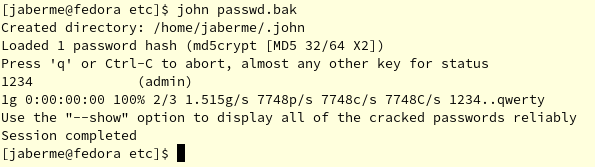
\includegraphics[scale=.8]{imagenes/john.png}
  \label{fig:pass}
\end{figure}

\begin{tcolorbox}[colback=red!5]
    En el caso de ester router el hash ha sido creado con \textbf{MD5} que es un algoritmo de hashing muy inseguro: \textbf{\textcolor{red}{primera vulnerabilidad}}.
\end{tcolorbox}

\subsubsection{Extracción selectiva}
Si recordamos, el fichero que contiene el firmware (figura~\ref{fig:rom}) nos decía que tenemos un conjunto de ficheros comprimidos con LZMA y que éste trozo de información se encuentra entre el bootloader y el sistema de archivos (este último ya lo hemos extraído y hemos visto que en el directorio /etc hay cosas interesantes, tanto que hemos practicado nuestras habilidades para romper contraseñas). Si queremos extraer la información comprimida con LZMA hemos de sacar este segmento de información binaria del archivo rom2.bin (que es nuestro archivo de prueba ya que es la copia de rom.bin que es el que hemos extraído del router). 

Para extraer el segmento LZMA sabemos que éste comienza en el byte 66560 y que continúa hasta el inicio del sistema de archivos (1049088). Sabemos que el segmento va, por tanto, de 66560 hasta 1049088. Es decir, el segmento ocupa 1049088y bytes - 66560 bytes= 982528 bytes. No tiene porqué estar todo repleto de información. Sólo sabemos que tengo que extraer 982528 bytes, y esto ya hemos visto cómo hacerlo con dd: 

\begin{verbatim}
dd if=rom2.bin skip=66560 count=982528 of=archivoComprimido.lzma bs=1
\end{verbatim}
\textbf{count} indica la cantidad de bytes a extraer a partir de 66560.

Como no sabemos cuantos de esos 982528 bytes contienen información y cuanto espacio hasta 1049088 hay con relleno, podemos usar el comando \emph{lzma} para eliminar esa parte inservible:

\begin{verbatim}
lzma -d < archivoComprimido.lzma > archivoFinal
\end{verbatim}

La salida de este comando indica que el archivo generado (archivoFinal) está corrupto, pero no es así. De hecho si lo examinamos con binwalk muestra todo su contenido, donde cabe destacar el segmento nombrado como \textbf{xz compressed data} (un segmento así llama la atención), los segmentos que hay antes son la versión del kernel y marcas CRC de comprobación de integridad. Otra información importante son los ASCII cpio archive que sirven como archivos de volcado (archivos de backup y restauración) en codificación ASCII (legibles). La figura~\ref{fig:lzma} muestra en mi terminal la secuencia de comandos que hemos descrito y los resultados: 

\begin{figure}[htpb]
     \caption{Extrayendo el otro segmento (LZMA)}
     \centering
     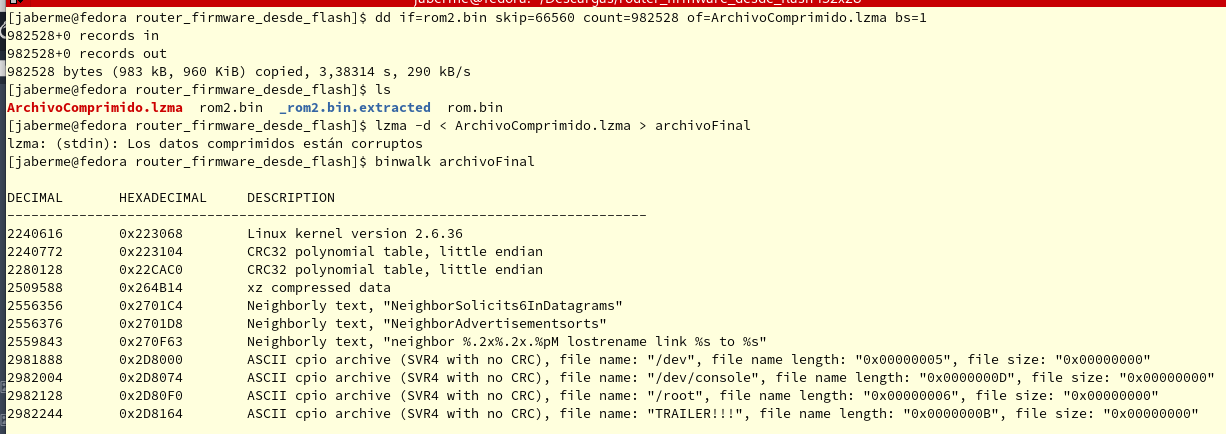
\includegraphics[scale=.38]{imagenes/lzma.png}
  \label{fig:lzma}
\end{figure}

Si analizamos la entropía de este segmento, podremos observar que al final del mismo (donde está la información legible en ASCII) la entropía está por debajo de 0.7 lo que quiere decir que esta información \textbf{no está ofuscada}.

\begin{figure}[htpb]
     \caption{Entropía de archivoFinal}
     \centering
     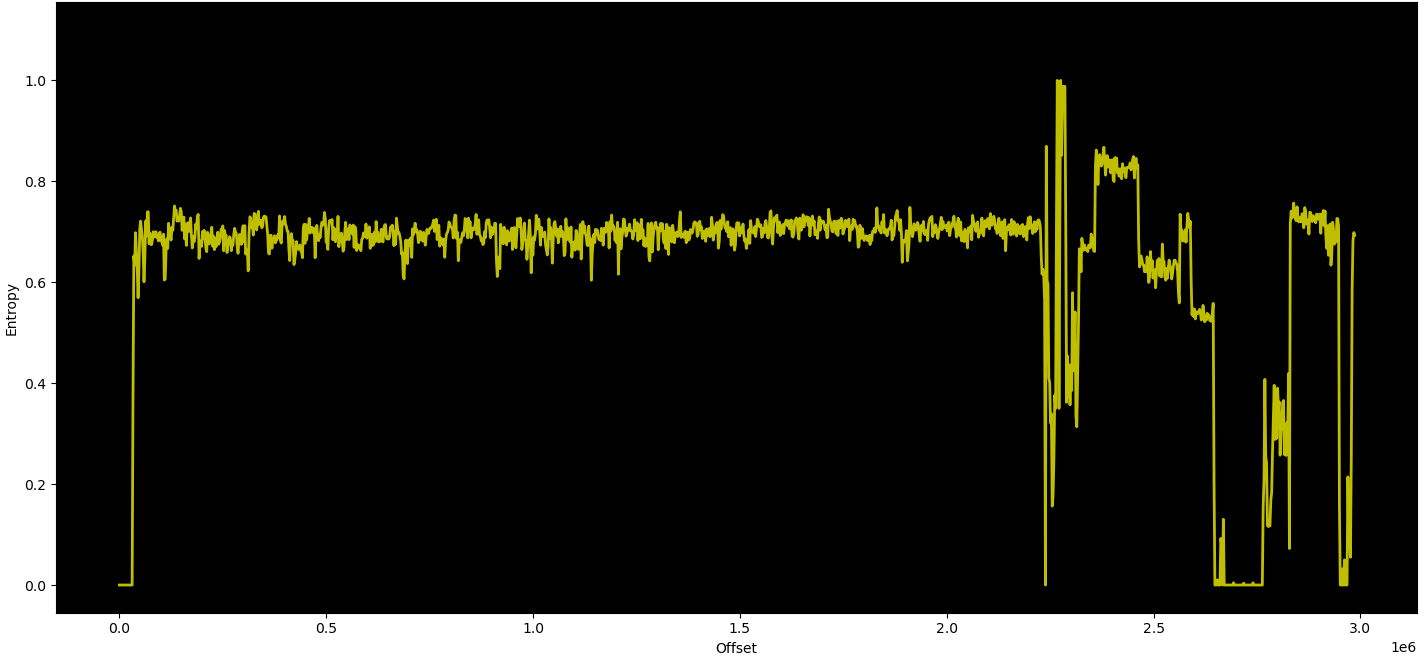
\includegraphics[scale=.35]{imagenes/entropia2.png}
  \label{fig:entropia2}
\end{figure}

\subsection{Explorando SquashFS:a la caza de claves de descifrado}

En el sistema de archivos (SquashFS) identificamos un directorio (/etc) que aparentemente tenía información interesante. Nos centramos en dos ficheros (passwd.bak que rompimos con JohnTheRipper) y había otro, llamado \textbf{default\_config.xml}. Cualquier archivo de configuración que encontremos nos puede dar muchísima información sobre el sistema. Si intentamos ver este fichero XML nos encontramos con 

\begin{minipage}{0.48\columnwidth}
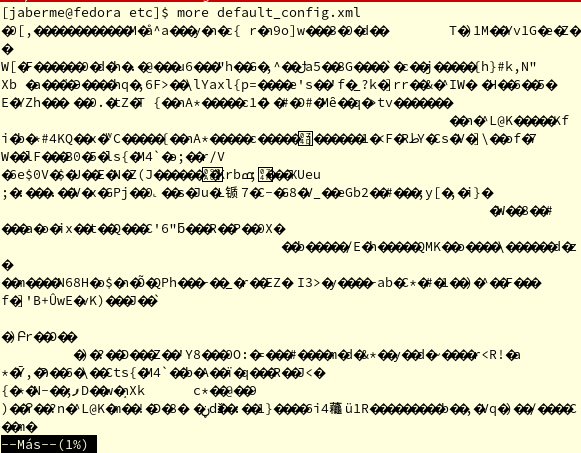
\includegraphics[scale=.3]{imagenes/defaultconfig.png}
\end{minipage}
\begin{minipage}{.5\columnwidth}
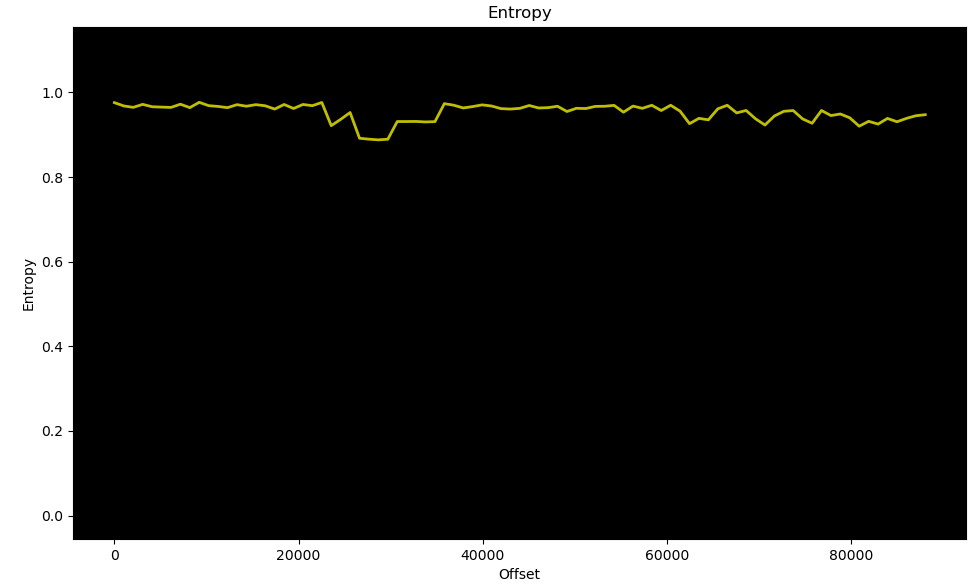
\includegraphics[scale=.25]{imagenes/entropy3.png}
\end{minipage}

Si entramos en /etc encontramos una plétora de archivos que podemos analizar, entre ellos binarios que parece que estan relacionados con el SoC MT7628. No obstante, el primer objetivo es \textbf{default\_config.xml} y al tratar de abrirlo (como hemos visto en las figuras anteriores) vemos que está cifrado (caracteres ilegibles) y una entropía altísima (>0.7). Si este fichero nos interesa, y no podemos abrirlo directamente, el paso a dar sería localizar qué programas del sistema operativo trabajan con éste XML (porque si los interceptamos podríamos ser capaces de intervenir la clave que usan para descifrar el contenido de \textbf{default\_config.xml}

\begin{verbatim}
grep -rnw ".." -e default_config.xml    
\end{verbatim}
\begin{itemize}
    \item r: recursivo 
    \item n: muestra número de línea
    \item w: buscamos coincidencias exactas con el patrón de búsqueda
\end{itemize}

El resultado es sólo uno y hace referencia a la librería \textcolor{red}{\textbf{../lib/libcmm.so}}, dentro del sistema de archivos del router localizamos a esta librería que usa el archivo \textbf{default\_config.xml}. Es razonable pensar que si éste archivo está usando \textbf{default\_config.xml} entonces en algún momento tendrá que descifrarlo para poder procesarlo. 

\subsection{GHIDRA (https://ghidra-sre.org/)}

Vamos a usar Ghidra (ver figura~\ref{fig:Ghidra}) para realizar ingeniería inversa sobre el archivo \emph{shared object(.so)} \textbf{\textcolor{red}{libcmm.so}}. 

\begin{figure}[htpb]
     \caption{Ghidra}
     \centering
     
\includegraphics[scale=.35]{imagenes/Ghidra.png}
  \label{fig:Ghidra}
\end{figure}

El primer paso será crear un proyecto nuevo a través de las opciones File-New Project. Debe configurarse como un proyecto no compartido (\emph{non shared project}). Y le damos un nombre (por ejemplo \emph{AnalisisRouter}). Arrastramos en ese proyecto a la librería que queremos examinar (nuestro .so -shared object-). El fichero libcmm.so se encuentra dentro del sistema de archivos root del router, concretamente en el directorio /lib. 

\begin{figure}[htpb]
     \caption{Ghidra: añadiendo libcmm.so}
     \centering
     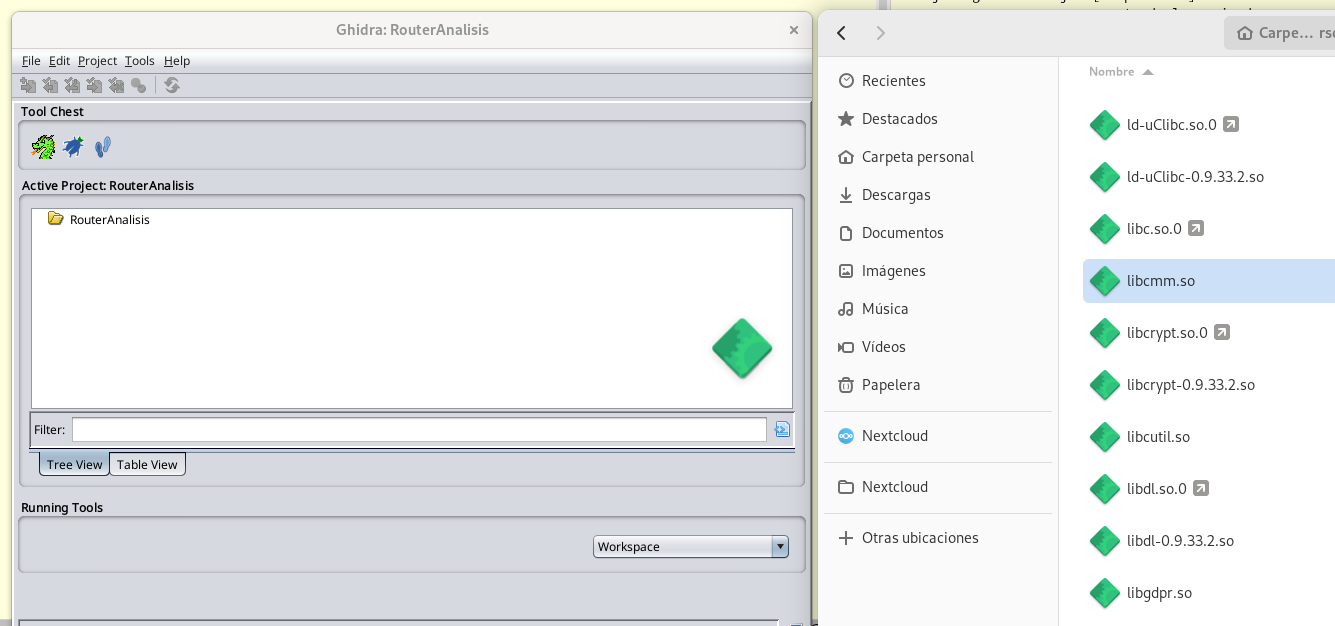
\includegraphics[scale=.35]{imagenes/RA.png}
  \label{fig:RA}
\end{figure}

En el proceso de inclusión del archivo Ghidra reconoce el tipo de ejecutable y no tenemos que indicarselo nosotros, tal como se puede ver en la figura~\ref{fig:RAfile}
\begin{figure}[htpb]
     \caption{Ghidra: añadiendo libcmm.so, reconoce el formato.}
     \centering
     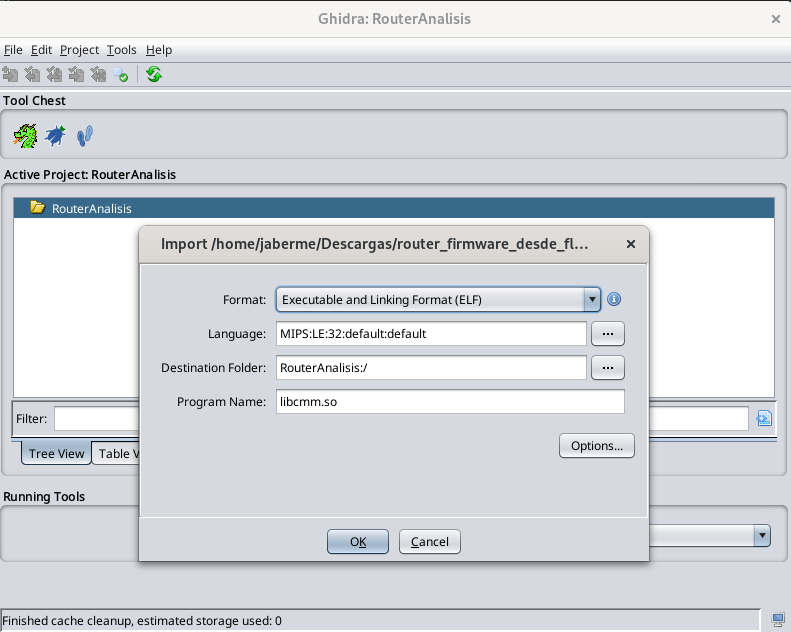
\includegraphics[scale=.5]{imagenes/RA_file.png}
  \label{fig:RAfile}
\end{figure}

Se identifica a la librería como un binario compilado para el procesador MIPS de 32 bits. Recordemos que el procesador que incorpora el router es un MIPS de 32 bits que opera con una frecuencia de 500 MHz. Los detalles extraídos por Ghidra se pueden consultar en la figura~\ref{fig:RArquitectura}. 

\begin{figure}[htpb]
     \caption{Ghidra: libcmmso, MIPS 32 bits.}
     \centering
     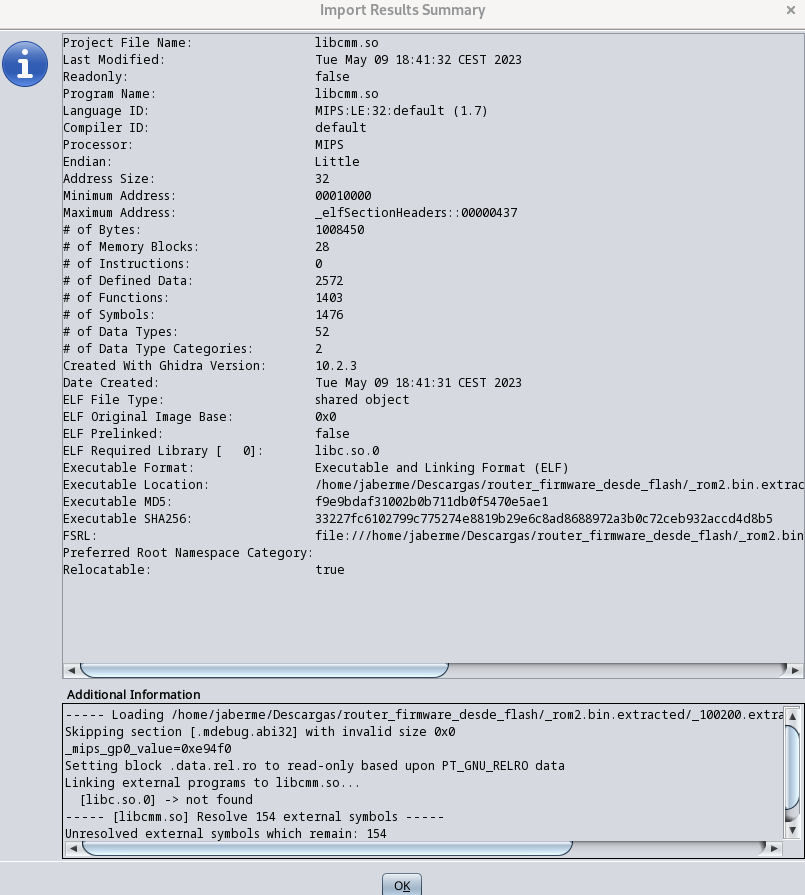
\includegraphics[scale=.5]{imagenes/RArquitecura.png}
  \label{fig:RArquitectura}
\end{figure}

Una vez que se ha importado el fichero, lo analizamos pulsando sobre el icono que representa a la cabeza de un dragón (figura~\ref{fig:RACabezaDragon}).

\begin{figure}[htpb]
     \caption{Ghidra: libcmmso, MIPS 32 bits.}
     \centering
     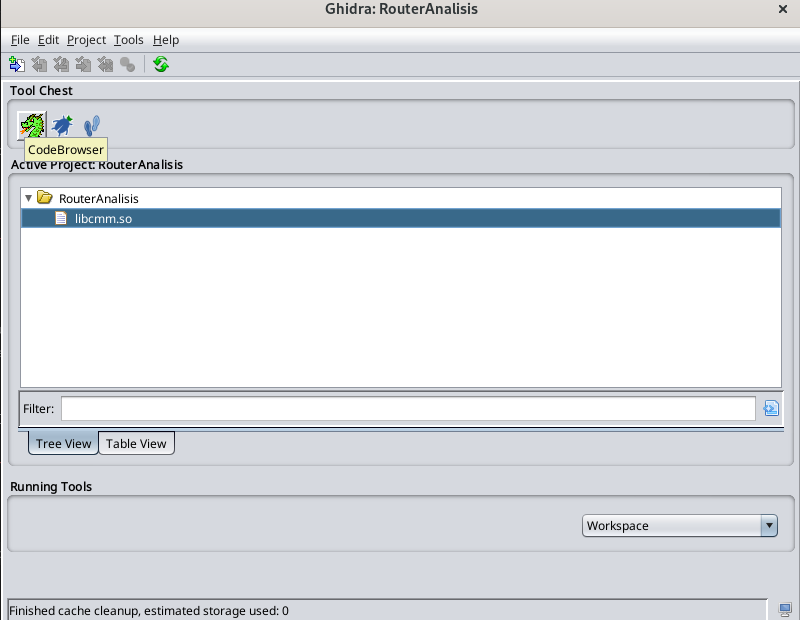
\includegraphics[scale=.5]{imagenes/RACabezaDragon.png}
  \label{fig:RACabezaDragon}
\end{figure}

Para realizar éste análisis nos basta con optar por las opciones por defecto. De modo que pulsamos \emph{Analyze} sin variar ninguna opción (ver figura~\ref{fig:licmmAnalisis}. 
\begin{figure}[htpb]
     \caption{Ghidra: libcmmso, inicio del análisis.}
     \centering
     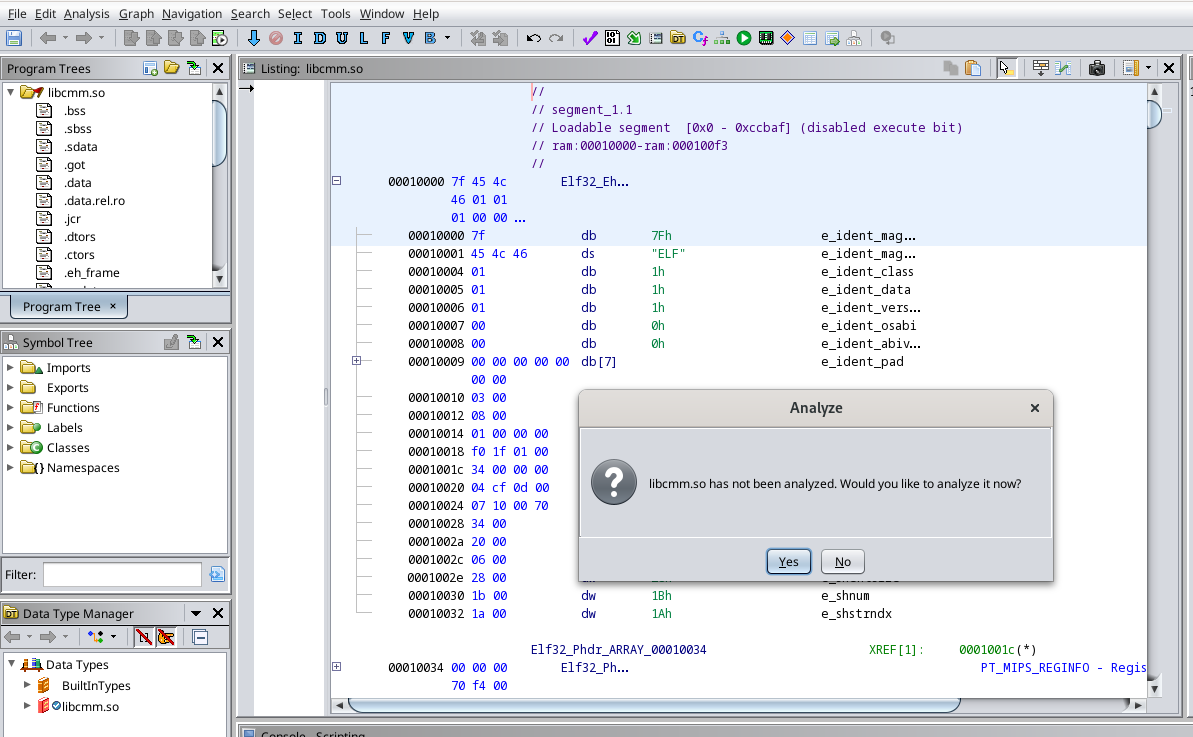
\includegraphics[scale=.35]{imagenes/licmmAnalisis.png}
  \label{fig:licmmAnalisis}
\end{figure}

En un primer análisis la opción por defecto nos resulta útil, si no podemos sacar mucha información optariamos por ampliar la gama de analizadores, pero por ahora los que están incluídos son suficientes. Cuando lanzamos el análisis hemos de considerar que éste puede tardar un rato en mostrarnos en la pantalla de Ghidra el \emph{desensamblado} de la librería. Cuando lo tengamos, y sin perder el foco en lo que estamos buscando (estamos buscando la relación entre este fichero y el que nos interesa desencriptar que es \emph{default\_config.xml}) lo primero que haremos será buscar esa cadena de texto en el código de la librería. Es decir, ¿dentro del código de libcmm.so hay referencias explícitas al xml \emph{default\_config.xml}? Si las hay, y como sospechamos debe haberlas, entonces se nos plantea la cuestión: si libcmm.so está accediendo a \emph{default\_config.xml}, lo tendrá que desencriptar primero ¿no? y si es así deberá tener la clave para hacerlo. Y a nosotros nos interesa esa clave para ver el contenido del archivo \emph{default\_config.xml}. Asi que una vez que tenemos el código de libcmm.so analizado vamos a buscar la cadena a través de \textbf{Search -> Program Text} (ver figura~\ref{fig:search}).

\begin{figure}[htpb]
     \caption{Ghidra: libcmmso, búsqueda de la cadena.}
     \centering
     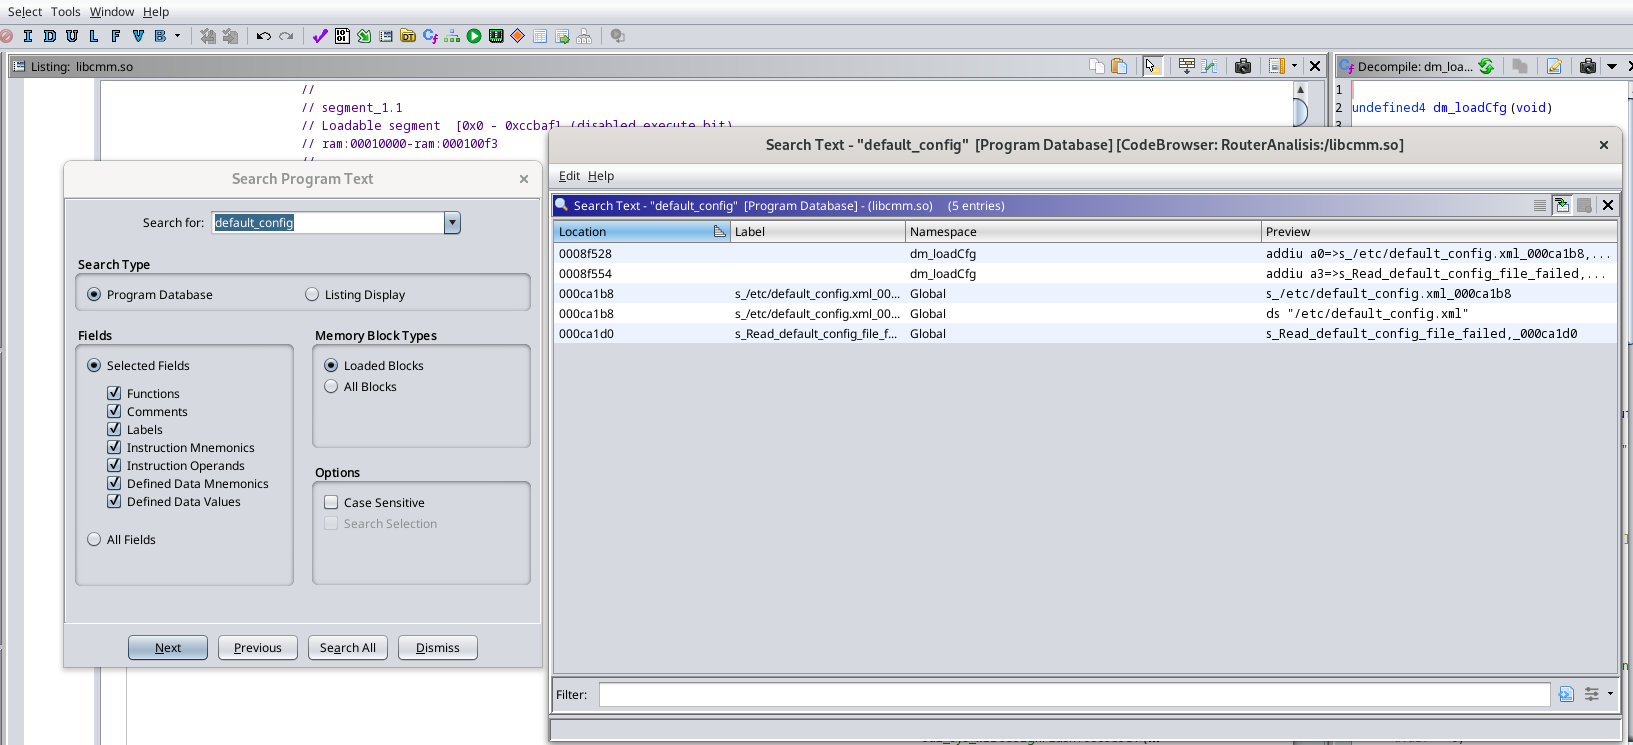
\includegraphics[scale=.25]{imagenes/search2.png}
  \label{fig:search}
\end{figure}

Las dos primeras opciones hacen referencia a código, por lo que son las primeras que analizaremos.  En estas primeras líneas de \emph{\textbf{dm\_loadCfg}} aparece la dirección de memoria donde se encuentra este código. Si pinchamos en la primera línea, nos lleva a esa posición (ver figura~\ref{fig:loadCfg}). 

\begin{figure}[htpb]
     \caption{Ghidra: dm\_loadCfg}
     \centering
     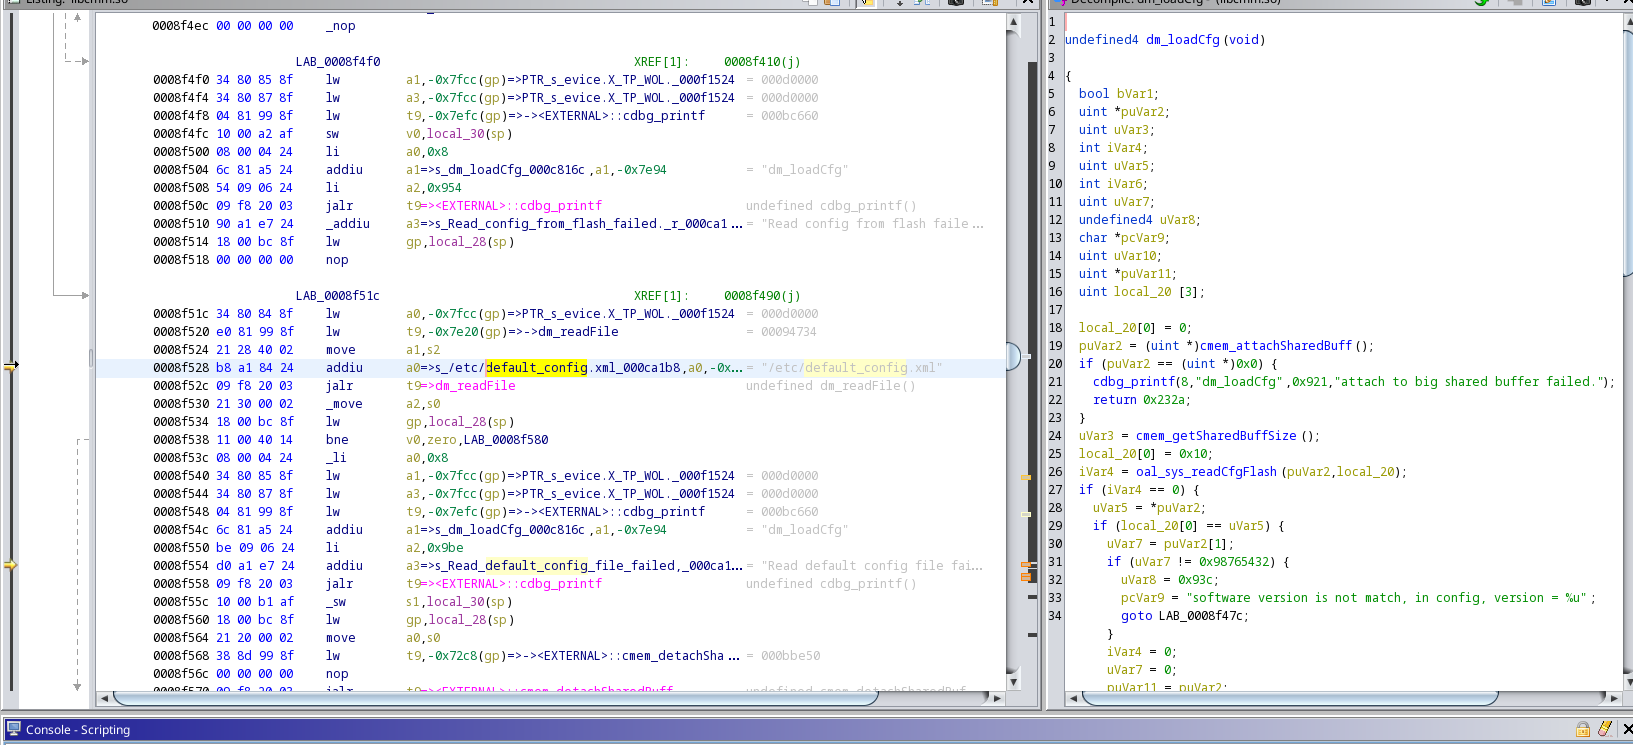
\includegraphics[scale=.25]{imagenes/loadCfg.png}
  \label{fig:loadCfg}
\end{figure}

Si nos movemos dentro de la función \textbf{dm\_loadCfg} (nos la muestra en el panel de la derecha) podemos ir viendo en un pseudo-c con algo más de legibilidad lo que hace esa función. Analizando esa función encontramos que se llama a otra función cuyo nombre es revelador: \textbf{\emph{dm\_decryptFile}}, esta función toma como entrada cuatro parámetros, pero no tenemos mucha más información para saber qué hacen de modo que pulsamos sobre el nombre de la función \textbf{\emph{dm\_decryptFile}} y trataremos de entender qué hace para desencriptar. En la figura~\ref{fig:dmDecryptFile}, al principio, podemos ver 8 bytes de datos copiados desde memoria en una variable llamada \textbf{auStack28}. Después se invoca a una función (\emph{cen\_desMinDo}, esta función es un \emph{wrapper} (es decir, una función que realmente se diseña para recoger parámetros pero que dentro está llamando a la función de descifrado) y para llamar a la función de descifrado (que se encuentra dentro de la librería libc.so) necesita proporcionar la clave. ¿Es posible que la clave esté almacenada en la variable \emph{auStack28}? Esta función tiene cinco parámetros, los cuatro primeros vienen desde dm\_decrypt. Y el parámetro final es justamente \textbf{auStack28}. Por lo que tiene toda la pinta de que esta sea la variable que almacena la clave para descifrar el archivo. 

\begin{figure}[htpb]
     \caption{Dentro de la función: dm\_loadCfg}
     \centering
     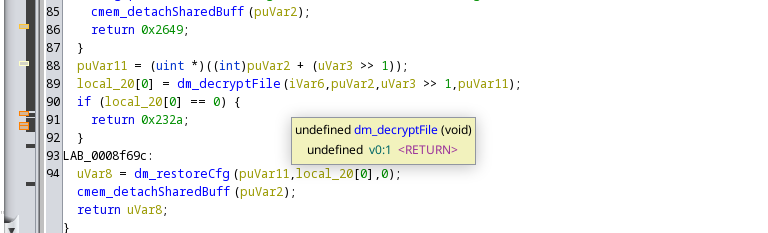
\includegraphics[scale=.25]{imagenes/dmDecrypt.png}
  \label{fig:dmdecrypt}
\end{figure}


\begin{figure}[htpb]
     \caption{Dentro de la función: dm\_decryptFile}
     \centering
     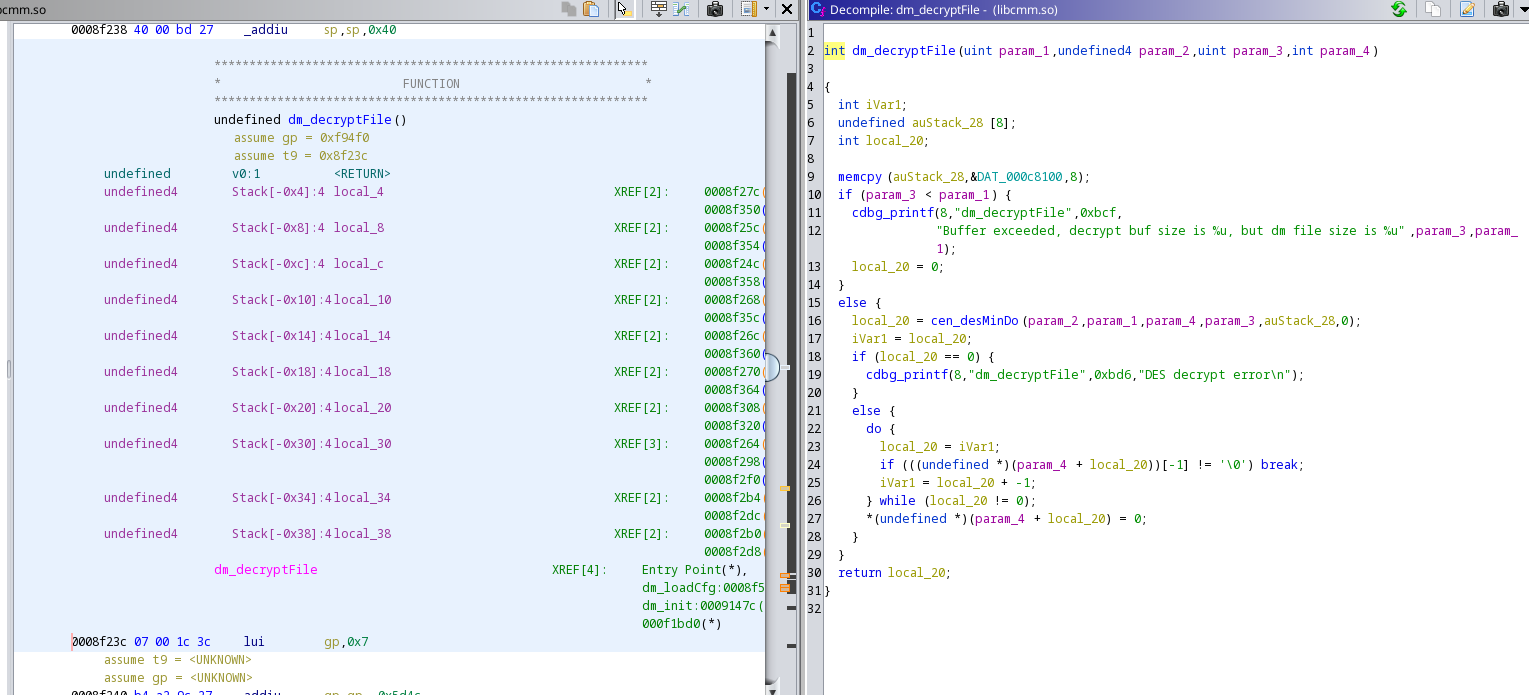
\includegraphics[scale=.25]{imagenes/decryptFile.png}
  \label{fig:dmDecryptFile}
\end{figure}

Parece razonable que lo siguiente que hagamos será dirigirnos a ver de dónde coge auStack28 los valores (de qué dirección de memoria), si estamos en lo cierto en esa dirección de memoria debería estar la clave de descifrado. En la figura~\ref{fig:memauStack28} se puede ver cómo podemos acceder al área de memoria desde la que se copia el contenido (con la función memcpy) en auStack28. 

\begin{figure}[htpb]
     \caption{Accediendo al area de memoria que nutre a auStack28}
     \centering
     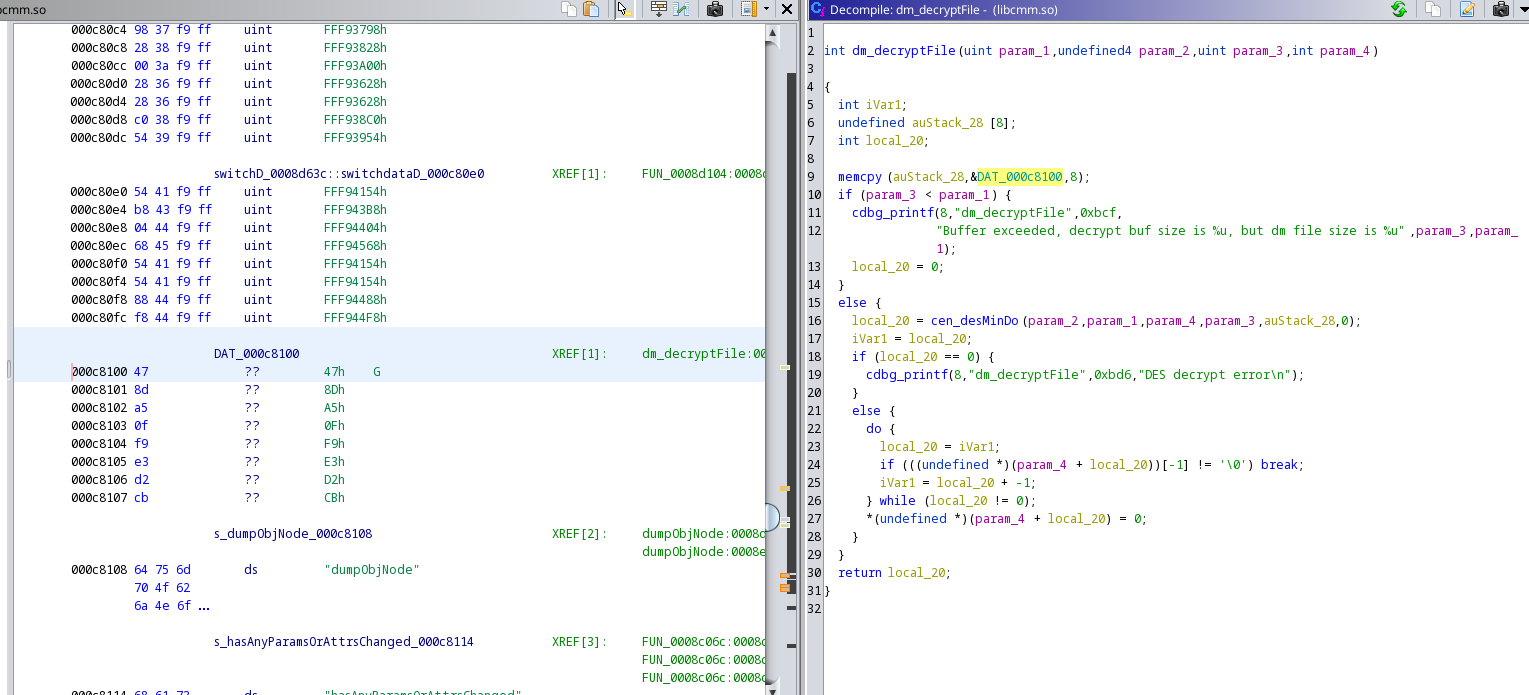
\includegraphics[scale=.35]{imagenes/memoria1.png}
  \label{fig:memauStack28}
\end{figure}

En esa posición del área de datos del programa podemos ver los 8 bytes que se copian en auStack28, \emph{\textbf{la clave de descifrado}} por tanto encontramos que aplicando técnicas de ingeniería inversa hemos descubierto otra puerta abierta y por tanto una (\textcolor{red}{segunda vulnerabilidad}). 

\subsubsection{Clave de descifrado}

Si estamos en lo cierto, hemos encontrado la clave. Para tratar de descifrar \textbf{config\_default.xml} vamos a usar \textbf{openssl}. 

\begin{tcolorbox}[colback=green!10]
    \textbf{openssl} es una herramienta de código abierto que contiene un conjunto de funciones muy útiles para la criptografía aplicada. Además, implementa los protocolos más conocidos y utilizados en computación, por lo que ofrece un amplio rango de alternativas útiles para programar. Se podría definir como un toolkit indispensable ya que reúne los algoritmos clave para forjar sistemas criptográficos de seguridad y certificados digitales SSL/TLS.   

    \textbf{La clave para descifrar} encontrada es \textbf{\textcolor{red}{478DA50FF9E3D2CB}}. Los parámetros de \textbf{openssl} que vamos a usar son: 

\begin{itemize}
    \item \textbf{-d} para indicar que vamos a descifrar.
    \item \textbf{-des-ecb} para indicar que el algoritmo a usar es DES (esto lo hemos visto en los comentarios del código de las funciones). 
    \item \textbf{-K} indica la clave que vamos a usar (\textbf{\textcolor{red}{478DA50FF9E3D2CB}}).
    \item \textbf{-in} indica el fichero a descifrar
    \item \textbf{-out} indica el nombre del archivo que vamos a crear con el contenido descifrado    
    \item \textbf{-provider} el cifrado DES-ECB es antiguo y no está incluído en el comando enc de openssl, hay que decirle que asumimos que es un comando antiguo y por eso hemos de recurrir a este parámetro.
\end{itemize}
\end{tcolorbox}

El comando que vamos a usar, por tanto, es :

\begin{tcolorbox}[colback=red!10]
openssl enc -d -des-ecb -in default\_config.xml -out descifrado.xml -K 478DA50FF9E3D2CB -provider legacy -provider default    
\end{tcolorbox}

Obtenemos un error al descifrar, pero podemos ignorarlo porque en el archivo descifrado tenemos el contenido (ver figura~\ref{fig:textoclaro}).

\begin{figure}[htpb]
     \caption{Fichero descifrado}
     \centering
     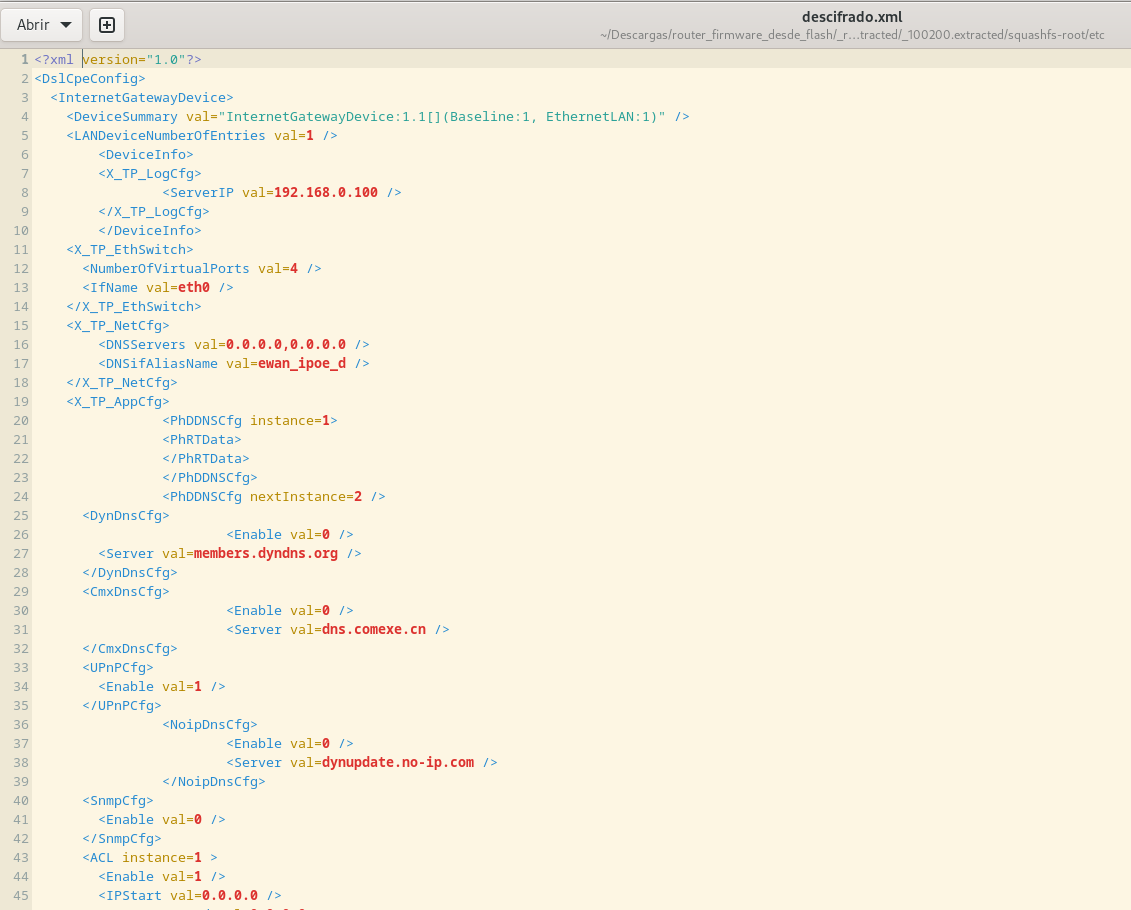
\includegraphics[scale=.45]{imagenes/textoclaro.png}
  \label{fig:textoclaro}
\end{figure}

En la documentación se aporta el fichero completamente descifrado para que se pueda ver información sensible como por ejemplo un PIN de un servicio de voicemail (123456), también encontramos un usuario por defecto para acceder a un cloud de almacenamiento (user: admin / password: admin) (el item xml es <StorageService>). 

Si se analiza el fichero descifrado se puede encontrar mucha información útil.

\subsection{Vulnerabilidades: Llamadas al sistema}
Llegados a este punto, se han realizado numerosas operaciones sobre el router: 

\begin{itemize}
    \item Se ha obtenido el firmware del router a través de diversos medios.
    \item Se ha extraído el sistema de archivos del linux que da soporte al router.
    \item Se ha revertido el hash de una contraseña usando JohnTheRipper
    \item Se ha realizado ingeniería inversa sobre una librería .so para extraer la clave con la que se ha cifrado un archivo con información sensible (claves por defecto, etc)
\end{itemize}

En una revisión más dedicada con Ghidra hemos observado un elemento importante contra la seguridad del router. En el panel de la izquierda (en Ghidra) tenemos la ventana \emph{Symbol tree} aquí se identifican los módulos, las funcoines, las clases, en definitiva todo lo usado por \textbf{libcmm.so}. La carpeta \textbf{imports} identifica funcionalidad que se encuentra fuera de libcmm (por ejemplo, la que proporciona el sistema operativo). ¿En qué función centrarse? No hay una norma. Pero en este caso nos ha llamado la atención que aparezca \textbf{\textcolor{red}{system}}, ver figura~\ref{fig:system}. A través del comando \emph{execute} se lanzan órdenes desde el router al sistema operativo (representado por la función System). 

\begin{figure}[htpb]
     \caption{System}
     \centering
     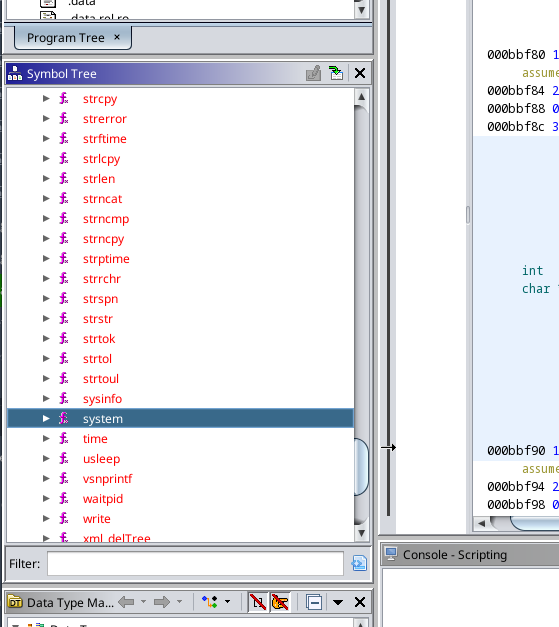
\includegraphics[scale=.45]{imagenes/system.png}
  \label{fig:system}
\end{figure}

En la siguiente figura~\ref{fig:exec} puede verse cómo en la ventana \emph{Function Call Trees} que se carga con las funciones accesibles desde dentro de System podemos ver dos muy interesantes: la primera es \textbf{updateFirmware} que sirve para actualizar el firmware del router y la segunda es \textbf{util\_execSystem} que es a través de la cual podemos acceder al sistema operativo que gestiona todo el router. Además, hay que recordar que cualquier llamada al sistema se realiza como \textbf{root, para ver esto basta ir al principio de este documento y ver que a la respuesta de whoami el usuario era admin}. Realizar llamadas al sistema con tal nivel de privilegio es un error desde el punto de vista de la seguridad es por tanto (\textbf{\textcolor{red}{vulnerabilidad}}). 

\begin{figure}[htpb]
     \caption{System: función execSystem}
     \centering
     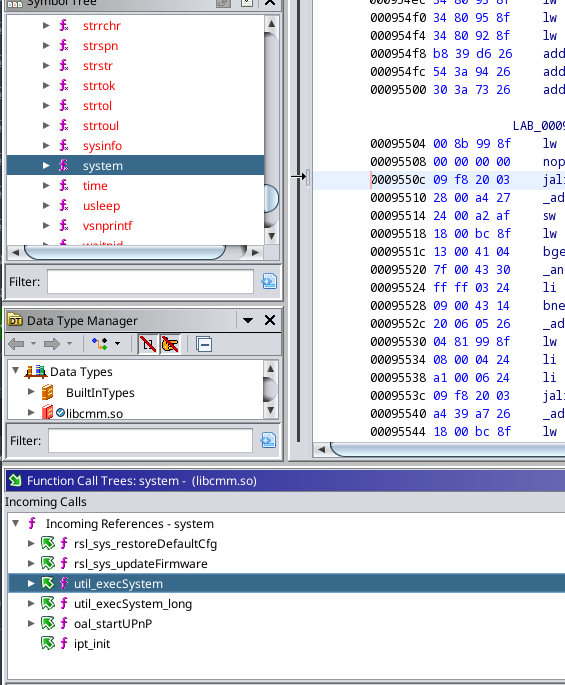
\includegraphics[scale=.4]{imagenes/exec.png}
  \label{fig:exec}
\end{figure}

Si nos desplazamos por el arbol de llamadas (Function call tree) veremos que hay decenas y decenas de llamadas al sistema a través de util\_execSystem. Escogiendo una de entre las que hay, por ejemplo \textbf{\textcolor{red}{oal\_ipt\_addBridgeIsolationRules}} podemos ver su función decompilada y cómo hace llamadas al sistema. La función recibe parámetros y realiza una llamada a System (Sistema Operativo) para ejecutar (internamente) el comando \textbf{iptables}, ver figura~\ref{fig:bridge}. Este comando está preparado para recibir la dirección ip a través de estos parámetros. Es muy probable que esta función se invoque desde la interfaz web del router que es quien ofrecerá al usuario la posibilidad de teclear la ip en cuestión desde la página de administración del router.  

\begin{figure}[htpb]
     \caption{Función oal\_ipt\_addBridgeIsolationRules}
     \centering
     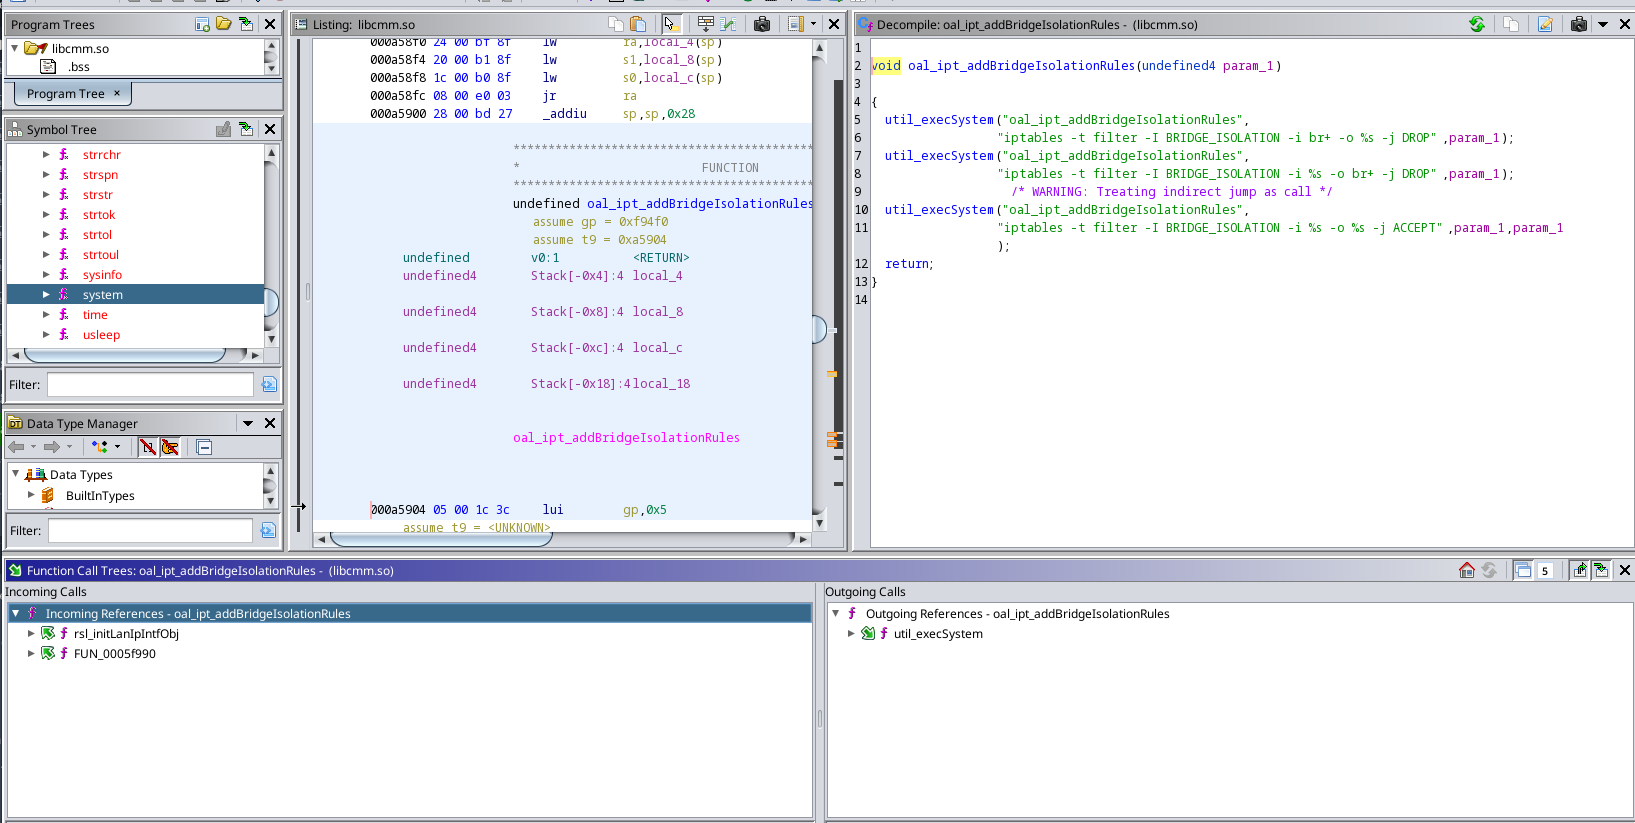
\includegraphics[scale=.30]{imagenes/bridge.png}
  \label{fig:bridge}
\end{figure}

El usuario, desde la página de administración del router especifica la dirección IP, esta web envía esta IP (\textbf{\textcolor{red}{SIN COMPROBAR (sin sanear) que realmente es una dirección IP}}. Esta dirección IP se incluye en un comando \emph{iptables} y se envía al sistema operativo del router (como usuario admin, no lo olvidemos). 

\subsubsection{Inyección de comandos}

¿Qué pasaría si en lugar de una dirección IP se enviara un comando específico al router? Pero claro, ¿cómo \emph{violar} un dato incluído desde la interfaz web si está no te permite teclear cosas a tu gusto? La respuesta es sencilla: necesitamos interceptar lo que el navegador al router:

\begin{itemize}
\item Conectamos nuestro ordenador a la misma red del router.
\item Accedemos a su IP a través del navegador.
\item Nos proporciona la página de configuración. 
\item Instalamos, por ejemplo, \textbf{Burp suite} en el ordenador.
\item Toda la información desde la web al router pasa por este \emph{proxy}.
\item Esa información queda retenida en \textbf{BurpSuite} modificamos el parámetro enviado desde la web al router  (porque lo tenemos parado en nuestro proxy) y lo enviamos.
\item El router ejecuta nuestro comando en lugar de aquel para el que estaba preparado.
\item Se habría logrado acceder vía web al sistema.
\end{itemize}

\begin{figure}[htpb]
     \caption{Inyección de comandos}
     \centering
     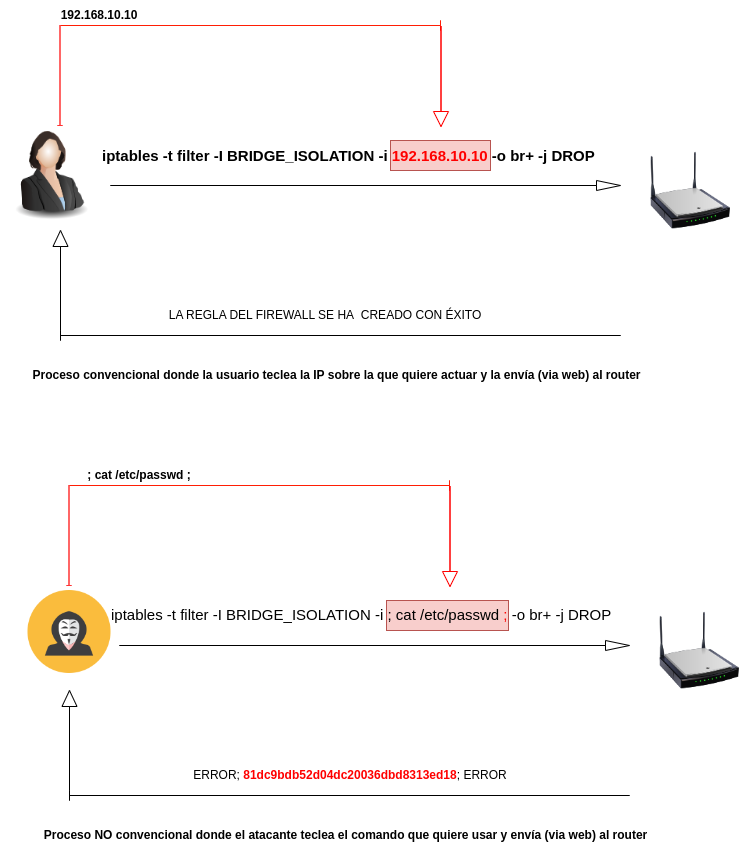
\includegraphics[scale=.65]{imagenes/tfg.png}
  \label{fig:tfg}
\end{figure}

La forma de hacer lo que se especifica en la figura~\ref{fig:tfg} es interceptando las comunicaciones entre el navegador del ordendor y el servidor web del router usando \textbf{BurpSuite} o similares. La figura~\ref{fig:burp} muestra el rol de BurpSuite como proxy. Éste intercepta las comunicaciones y te premite cambiar parámetros. Si escribimos una IP enviamos el formulario web al router y en lugar de que éste llegue directamente lo hacemo pasar por \textbf{BurpSuite}, ahí cambiamos la IP por un comando y ya estaríamos en disposición de someter el router a nuestra voluntad.

\begin{figure}[htpb]
     \caption{BurpSuite}
     \centering
     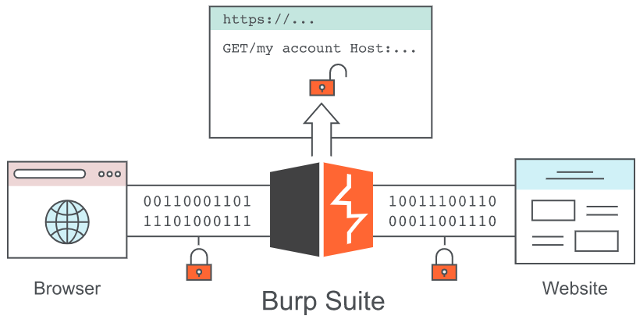
\includegraphics[scale=1]{imagenes/burp_suite.png}
  \label{fig:burp}
\end{figure}

\section{Más recursos}

\begin{tcolorbox}[enhanced, dropshadow, title=Reversing a tope, colback=blue!10]
    \begin{itemize}
        \item \href{Introducción a la ingeniería inversa en dispositivos empotrados.}{https://voidstarsec.com/blog/intro-to-embedded-part-1}
    \end{itemize}
    
\end{tcolorbox}



\printbibliography

\end{document}
